% $Id$
\documentclass[10pt]{article}
\usepackage{epsfig}
\usepackage{dcolumn}

\def\numpackages{30}
\def\numlines{2 million}
\def\numlinesexact{nearly 2 million}
\def\numlinesncnbexact{about 1.4 million}

\newcommand{\pkg}[1]{\textsf{#1}}

\newcommand{\file}[1]{\texttt{#1}}

% the "fullpage" package does almost the same thing
% as the below lines-- it doesn't make things quite as
% tall or wide, but is generally what I use
% \usepackage{fullpage}
\marginparwidth 0pt
\oddsidemargin  0pt
\evensidemargin 0pt
\marginparsep 0pt
\topmargin   0pt
\headsep 0pt
\headheight 0pt
\textwidth   6.5 in
\textheight  9 in

\renewcommand{\floatpagefraction}{.8} %default .5
% Avoid putting all figures at end of text.
\renewcommand{\textfraction}{.1}  % .2 is the default
\renewcommand{\topfraction}{.9}   % .7 is the default

\begin{document}
% \bibliographystyle{plain}
\bibliographystyle{alpha}

\title{An Empirical Analysis of C Preprocessor Use}

\author{Michael D. Ernst%
  \and Greg J. Badros%
  \thanks{Supported by a National Science Foundation
    Graduate Fellowship. Any opinions, findings, conclusions, or
    recommendations expressed in this publication are those of the
    author, and do not necessarily reflect the views of the National
    Science Foundation.}
  \and David Notkin}

\date{% Technical Report UW-CSE-97-04-06 \\
Department of Computer Science and Engineering \\
University of Washington \\
Box 352350, Seattle, WA  98195-2350  USA \\
{\small \{{\tt mernst},{\tt gjb},{\tt notkin}\}{\tt @cs.washington.edu}} \\
11 October 1997}  

\maketitle

\begin{abstract}
  The C programming language is intimately connected to its macro
  preprocessor Cpp.  This relationship hinders tools built to engineer C
  programs, such as compilers, debuggers, call graph extractors, and
  translators.  Most tools make no attempt to analyze macro usage, but simply
  preprocess their input, which has a number of negative consequences.  In
  order to determine how the preprocessor is used in practice, and the
  feasibility of automatic analysis of preprocessor use, this paper
  analyzes {\numpackages} packages comprising {\numlines} lines of publicly
  available C code.  We determine the incidence C preprocessor usage which
  is complex, potentially problematic, or inexpressible in in terms of
  other C or C++ language features.
[[We also came up with the list of things to investigate; and along the way
we taxonomized some stuff, which is also a contribution.]]

  We particularly note data that are
  material to the development of tools for C or C++, including translating
  from C to C++ to reduce preprocessor usage.  The results are of interest
  to language designers, tool writers, programmers, and software engineers.
\end{abstract}

\bigskip

\section{Introduction}

The C programming language~\cite{ansi} is incomplete without its macro
preprocessor, Cpp~\cite[Ch.~3]{Harbison91}, which supplies such facilities
as file inclusion, definition of constants and macros, and conditional
compilation.  While disciplined use of the preprocessor can reduce
programmer effort and improve portability, performance, or readability, Cpp
is widely viewed as a source of difficulty for understanding and
transforming C programs.  Because of Cpp's lack of structure\,---\,its
inputs and outputs are raw token streams\,---\,Cpp is very flexible, but
lends itself to arbitrary source code manipulations that complicate
understanding of the program by both software engineers and tools.  In the
worst case, the preprocessor makes merely determining the program text as
difficult as determining the output of an ordinary program.  The designer
of C++, which shares C's preprocessor, also noted these problems:
``Occasionally, even the most extreme uses of Cpp are useful, but its
facilities are so unstructured and intrusive that they are a constant
problem to programmers, maintainers, people porting code, and tool
builders.''~\cite[p.~424]{Stroustrup-DesignEvolution}

While much has been written about Cpp's potential pitfalls, no previous
work has examined actual use of the C preprocessor to determine whether it
presents a practical or merely theoretical obstacle to program
understanding, analysis, and transformation.  This paper fills that gap by
examining CPP use in {\numpackages} programs comprising {\numlines} lines
of source code.

We identified a number of potential pitfalls proceeding from preprocessor
use, including
\begin{description}
\item[high total use]  heavy use of either macro substitution or
  conditional compilation can overwhelm a human or tool; particularly
  problematic are lines that depend on many macros or macros that control
  many lines
\item[complicated bodies]  a macro body need not expand to a complete
  C syntactic entity (like a statement or expression)
\item[extra-linguistic features]  a macro body may exploit features of
  the preprocessor not available in C, such as stringization, token
  pasting, or use of free variables
\item[multiple definitions]  uncertainty about the expansion of a macro
  prevents knowledge of the actual program text; even more problematically,
  two definitions of a macro may be incompatible, for instance if one is a
  statement and the other expands to an expression or type
\item[macro pitfalls]  macros introduce new varieties or programming
  errors, such as function-like macros that fail to swallow a following
  semicolon and macros that fail to parenthesize, or side-effect, uses of
  formal variables
\item[inconsistent usage]  a macro used both for conditional
  compilation and to expand code is harder to understand than one used just
  for one purpose or the other
\item[mixed tests]  a single Cpp conditional may test conceptually
  distinct, unrelated conditions, making it difficult to perceive the
  intention
\item[variation in use]  if there is no clear pattern of use, or
  commonly-repeated paradigms, then no obvious point of attack presents
  itself
  %% No pattern according to package size, relative or absolute Cpp use, etc.
\end{description}
We report in detail on each of these aspects of preprocessor use,
indicating which appear to be innocuous in practice (that is, the
problematic uses appear only infrequently) and which may prove problematic
for software engineers.  We also present new taxonomies of macro body
expansions, macro feature usage, macro pitfalls, and conditional
intentions.  These taxonomies improve on previous work by being more
detailed and more accurately reflecting actual use.

Sections~\ref{sec:first-content-section}--\ref{sec:last-content-section}
present the bulk of these results.  Section~\ref{sec:methodology} describes
our experimental methodology.  Section~\ref{sec:conclusion} discusses the relevance of the research,
suggests techniques for mitigating the negative impact of Cpp on program
understanding, and discusses avenues for future work, while
section~\ref{sec:related} discusses related work.
The remainder of this section [[does some stuff]].

[[Point reader at conclusion/summary of results, at end of paper (and write
that!).]]

% \subsection{Outline}
% 
% The remainder of this paper is organized as follows.
% 
% Section~\ref{sec:directives} reports the percentage of original C source
% code lines that are preprocessor directives, including a breakdown of the
% frequency of specific directives such as {\tt \#define}.  C programs
% commonly have preprocessor directives as over 10\% of their total lines,
% and over 20\% of the lines were directives in 3 of the {\numpackages}
% packages.
% 
% Section~\ref{sec:usage} reports how often each macro is defined and
% expanded.   Identifiers tend to be {\tt \#define}d relatively few times
% (96\% of macro identifiers had three or fewer definitions).  Many packages
% also have a significant number of macros that are never expanded, even
% disregarding system and library header files.
% 
% Section~\ref{sec:categorization} categorizes macro definitions according to
% their expansions; for example, macros may simply define a preprocessor
% symbol, define a literal, expand to a statement, etc.  We were particularly
% interested in determining the frequency of use of macros that are difficult
% to convert to other language features, such as those that string together
% characters as opposed to manipulating lexemes or syntactic units (less than
% one third of one percent of all macro definitions),
% those that expand to partial syntactic units such as unbalanced
% braces or partial declarations (half of one percent), and others not 
% directly expressible in the programming language (about four percent).
% 
% Section~\ref{sec:conclusion} discusses the relevance of the research,
% suggests techniques for mitigating the negative impact of Cpp on program
% understanding, and discusses avenues for future work, while
% section~\ref{sec:related} discusses related work.


[[Does anyone care about this?
Another niche already filled by our tool is that of a ``macro lint''
program which warns of potentially dangerous (or non-standard) uses of Cpp.
And, we wrote CPPP.]]



% In order to assess the practical difficulty of understanding uses of CPP
% (and the potential for replacement by other language constructs), 





Overall, our analysis confirms that the C preprocessor is used in
exceptionally broad and diverse ways, complicating the development of C
programming support tools.  On the other hand, the analysis also convinces
us that, by extending our analysis framework with some class type
inferencing techniques (similar to those used for C to C++
translation~\cite{Siff-fse96} and for program
understanding~\cite{OCallahan-icse97}), we can take significant
steps towards a tool that usefully converts a high percentage of Cpp code
into C++ language features.  We are interested not in translations
that merely allow a C program to be compiled by a C++ compiler (which is
usually easy, by intentional design of C++) but those that take advantage
of the added richness and benefits of C++ constructs.

[[Inane, content-free.  Must die.]]
In terms of the complexity of preprocessor usage, the results reported here
contain both good news and bad.  By far
the largest number of macro definitions and uses are relatively simple, of
the variety that a programmer could understand without undue effort (although
perhaps requiring tedious work) or that a relatively unsophisticated tool
could understand (although in practice very few even try).  Despite the
preponderance of innocuous macros, the preprocessor is so heavily used that
the remaining ones are numerically significant.  It is precisely these
macros that are mostly likely to cause difficulties, and there are enough
of them to be problematic in practice and to make the effort of
understanding, annotating, or eliminating them worthwhile.


\subsection{Coping with Cpp}

Tools\,---\,and, to a lesser degree, software engineers\,---\,have three
options for coping with Cpp.    They may ignore preprocessor directives
(including macro definitions) altogether, accept only post-processed code
(usually by running Cpp on their input), or attempt to emulate the
preprocessor.

Ignoring preprocessor directives is an option for approximate tools, such
as those based on lexical or approximate parsing techniques.  Accurate
information about function extents, scopes, declared variables and
functions, and other aspects of a program requires addressing the
preprocessor.

Operating on post-processed code, the most common strategy, is simple to
implement, but then the tool's input differs from what the
programmer sees.  Even when line number mappings are maintained, other
information is lost in the mapping back to the original source code.
For instance, source-level debuggers have no symbolic names or types
for constants and functions introduced via {\tt \#define}, nor can tools
trace or set breakpoints in function macros, as they can for ordinary
functions (even those that have been inlined~\cite{Zellweger83:TR}).
As another example, Siff
and Reps describe a technique that uses type inference to produce
C++ function templates from C; however, the input is ``a C program
component that $\ldots$ has been preprocessed so that all include
files are incorporated and all macros
expanded~\cite[p.~145]{Siff-fse96}.''  Such preprocessing may limit
the readability and reusability of the resulting C++ templates.  As
yet another related example, call graph extractors generally work in
terms of the post-processed code, even when a human is the intended
consumer of the call graph~\cite{Murphy-icse18}.  Some tools even
leave the software engineer responsible for inferring the mapping between the
original and the post-processed source, which is an undesirable and
error-prone situation.

A tool that first preprocesses code, or takes already-preprocessed code as
input, cannot be run on a non-syntactic program or one that will not
preprocess on the platform on which the tool is being run.  These
constraints complicate porting and maintenance, two of the situations in
which program understanding and transformation tools are most likely to be
needed.  Additionally, a tool supplied with only one post-processed
instantiation of the source code cannot reason about the program as a
whole, but only about that version that results from one particular set of
preprocessor variables.  For instance, a bug in one configuration may not
be discovered despite exhaustive testing of other configurations that do
not incorporate particular code or do not admit particular execution paths.

The third option, emulating the preprocessor, is fraught with difficulty.
Macro definitions consist of complete tokens but need not be complete
expressions or statements.  Conditional compilation and alternative macro
definitions lead to very different results from a single original program
text.  Preprocessing adds complexity to an implementation, which must trade
off performing preprocessing against maintaining the code in close to its
original form.  Extracting structure from macro-obfuscated source is not a
task for the faint-hearted.  Despite these problems, in many situations
only some sort of preprocessing or Cpp analysis can produce useful answers.

All three approaches would be unnecessary if programs did not use
preprocessor directives.  This is exactly what Stroustrup suggests:
\begin{quote}
  I'd like to see Cpp abolished.  However, the only realistic and
  responsible way of doing that is first to make it redundant, then
  encourage people to use the better alternatives, and {\em then\/}\,---\,years
  later\,---\,banish Cpp into the program development environment with the
  other extra-linguistic tools where it
  belongs~\cite[p.~426]{Stroustrup-DesignEvolution}.
\end{quote}
C++ contains features\,---\,such as constant variables, inline functions,
templates, and reference parameters\,---\,that obviate many uses of Cpp.
Thus, translation to C++ is a path for partial elimination of Cpp.
This study indicates the
feasibility\,---\,and our framework for analyzing preprocessor usage
provides a basis for the development\,---\,of an automatic translator with
two attractive properties.  It would take as input C programs complete with
preprocessor directives, and it would map many uses of directives into C++
language features.  (It is not 
practical to eliminate all uses of Cpp.  For example, C++ currently
provides no replacement for the {\tt \#include} directive, or for
stringization or pasting.  Macros that cannot be eliminated might be
annotated with their types or 
effects on parser or program state, so that even tools that do no Cpp
analysis can operate correctly on such programs.)

[[Where do these two points go?]]

Another niche already filled by our tool is that of a ``macro lint''
program which warns of potentially dangerous (or non-standard) uses of Cpp.

And, we wrote CPPP.

%O'Callahan and Jackson also use type
%inference, although for program understanding rather than translation;
%they, too, apply their techniques to post-processed
%code~\cite{OCallahan-icse97}.


\subsection{Cpp: not all bad}

[[This section is out of place and horrible.  Where should the information
go?]]

Despite its evident shortcomings, Cpp is a useful and often necessary
adjunct to C, for it provides capabilities unavailable in the language or
its implementations.  Cpp permits definition of portable language
extensions that can define new syntax, abbreviate repetitive or complicated
constructs, or eliminate reliance on a compiler implementation to
open-code (inline) functions, propagate symbolic constants, eliminate dead
code, and short-circuit constant tests.  The latter guarantees are
especially valuable for compilers that do a poor job optimizing or when the
programmer wishes to override the compiler's heuristics.  Cpp also permits
system dependences to be made explicit and tested, resulting in a clearer
separation of concerns.  Finally, Cpp permits a single source to contain
multiple different dialects of C; a frequent use is to support both
K\&R-style and ANSI-style declarations.

%% NEED A REFERENCE TO DEBUGGER HERE!
%% also mention Emacs hide-ifdef mode

Our long-term goal is not to take these useful features away from
programmers, but to reduce Cpp use, making programs easier for humans to
understand and tools to analyze.






\section{Methodology}
\label{sec:methodology}

We analyzed {\numpackages} publicly-available software packages which
represent a mix of application domains, authors, programming styles, and
sizes.  Some are interactive, while others are not, and some are graphical
while others are text-based, command-line applications.
Figure~\ref{fig:packages} describes the packages and lists their sizes in
terms of physical lines (newline characters) and non-comment, non-blank
(NCNB) lines.  The NCNB figure disregards lines consisting of only comments
or whitespace, as well as lines in a conditional that cannot evaluate to
true (such as {\tt \#if 0}, which is frequently used to comment out code).  The
remainder of our analysis uses the NCNB length, which more accurately
reflects the amount of source code.

\begin{figure}
\centering
{% ``\small'' here does have an effect, despite previous comment to the contrary
  \small
  \setlength{\tabcolsep}{.25em}
  \begin{tabular}{|l|r|r|r|r|r|r|r|} \hline
Package & Version & Physical lines & NCNB lines & Files & Description \\ \hline
bash & 1.14.7 & 55079 & 38111 & 128 & Command shell  \\ \hline
bc & 1.03 & 11193 & 8026 & 28 & Desktop calculator  \\ \hline
bison & 1.25 & 10799 & 7260 & 29 & Parser generator  \\ \hline
cvs & 1.9 & 56902 & 39273 & 108 & Revision control system  \\ \hline
emacs & 19.34 & 132929 & 89335 & 115 & Text editor \\ \hline
flex & 2.5.3 & 15475 & 10648 & 17 & Scanner generator  \\ \hline
fvwm & 2.0.43 & 42953 & 32517 & 111 & Window manager  \\ \hline
gawk & 2.15.6 & 21291 & 14963 & 22 & GAWK interpreter  \\ \hline
gcc & 2.7.2.2 & 346395 & 235237 & 193 & C and C++ compiler \\ \hline
genscript & 1.3.2a & 11546 & 7969 & 23 & Text-to-PostScript converter  \\ \hline
ghostview & 1.5 & 11214 & 8762 & 22 & PostScript previewer  \\ \hline
gnuchess & 4.0pl77 & 15183 & 12532 & 28 & Chess player  \\ \hline
gnuplot & 3.50.1.17 & 40800 & 30247 & 71 & Graph plotter  \\ \hline
gs & 5.10 & 182933 & 127136 & 594 & PostScript interpreter  \\ \hline
gzip & 1.2.4 & 8148 & 5186 & 19 & File compressor  \\ \hline
m4 & 1.4 & 15316 & 9386 & 22 & Macro expander  \\ \hline
mosaic & 2.6 & 82791 & 55194 & 190 & WWW browser \\ \hline
perl & 5.003 & 69722 & 61090 & 82 & Perl interpreter  \\ \hline
plan & 1.7.1 & 30894 & 24439 & 77 & Schedule planner  \\ \hline
rasmol & 2.5 & 21863 & 17845 & 23 & Molecular visualization \\ \hline
rcs & 5.7 & 18444 & 12134 & 29 & Revision control system  \\ \hline
remind & 3.00.16 & 15611 & 11086 & 29 & Schedule reminder  \\ \hline
workman & 1.3 & 13486 & 9928 & 58 & Audio CD player  \\ \hline
xfig & 3.1.4 & 52400 & 41259 & 118 & Drawing program  \\ \hline
zephyr & 2.0.4 & 42008 & 28016 & 240 & Notification system  \\ \hline
zsh & 3.0.5 & 47244 & 36298 & 75 & Command shell  \\ \hline
Total &   & 1372619 & 973877 & 2451 &   \\ \hline
\end{tabular}

}
\caption{Analyzed packages and their sizes.  NCNB lines are non-comment,
  non-blank lines.}
\label{fig:packages}
\end{figure}

Before performing our analysis, we ran {\tt configure} or the equivalent on
each package in order to prepare it for compilation.  This creates various
header files (such as \file{configure.h}).  Our analysis works in the
absence of this step, but warns about uses of never-defined macros and
underreports some values related to those missing definitions.  We did
not, however, compile the packages; our analysis does not require that the
package be compilable (or even that the preprocessor be able to run on it).

We generated a list of all the C files in the package (both code and header
files).  In general, these have extensions like \file{.c}, \file{.h},
\file{.cc}, \file{.cpp}, \file{.hxx}, etc.  We removed files with such
extensions that don't actually contain valid C, and added others which were
{\tt \#included} by valid C files (some included files had extension
\file{.def}).

We analyzed all the C files in the package, as well as every file {\tt
\#include}d by any of those, primarily library header files.  We
took care to include as many libraries as possible so as not to overlook
those definitions.  However, the figures reported in this paper always omit
all macros defined only in libraries, as well as all macro uses in
libraries.  This prevents libraries from 
swamping the characteristics of the package code, which is our focus in
this study.  The programmer generally has no control over libraries and
their header files, and may not even know whether a library symbol is
defined as a macro or a true function or variable.  Finally, we assume that
library macros are carefully written to behave correctly and robustly
(sadly, we discovered this not to always be true in practice; an
analysis of library macros is outside the scope of this report).

Our analysis is a true whole-program analysis; rather than preprocessing the
code and examining just one configuration, we examine all possible code and
ignore no possible  conditional compilation conditions (though we do skip
over those which can be statically proven to be false).   As a result, this
analysis is more thoroughgoing than traditional ``whole-program'' analyses.

[[We merge different cpp branches in the code wherever possible.  Discuss
this a bit.]]

We perform approximate parsing because the input is not a valid C program;
as a result, we miss some constructs, but we can cope with uncompilable C
and with partial constructs in conditional compilation branches.  Our tool
includes parsers for expressions, statements, and declarations.

We performed our analysis via a collection of Perl scripts, totaling
approximately 11,000 lines (7,000 NCNB lines).  The raw data, which
includes considerable data not reported here, and the programs used to
generate and manipulate them, are available from the authors.







\section{Occurrence of preprocessor directives}
\label{sec:directives}
\label{sec:first-content-section}

Figure~\ref{fig:directives-breakdown} shows how often preprocessor
directives appear in the programs we analyzed.  Each group of bars in the
figure represents the percentage of non-comment, non-blank (NCNB) lines
attributed to the specified category of directives, with each individual
bar showing the percentage for a specific package.  Conditional compilation
directives ({\tt \#if}, {\tt \#ifdef}, {\tt \#ifndef}, {\tt \#else}, {\tt
\#elif}, {\tt \#endif}) are grouped together.

\begin{figure}
\centerline{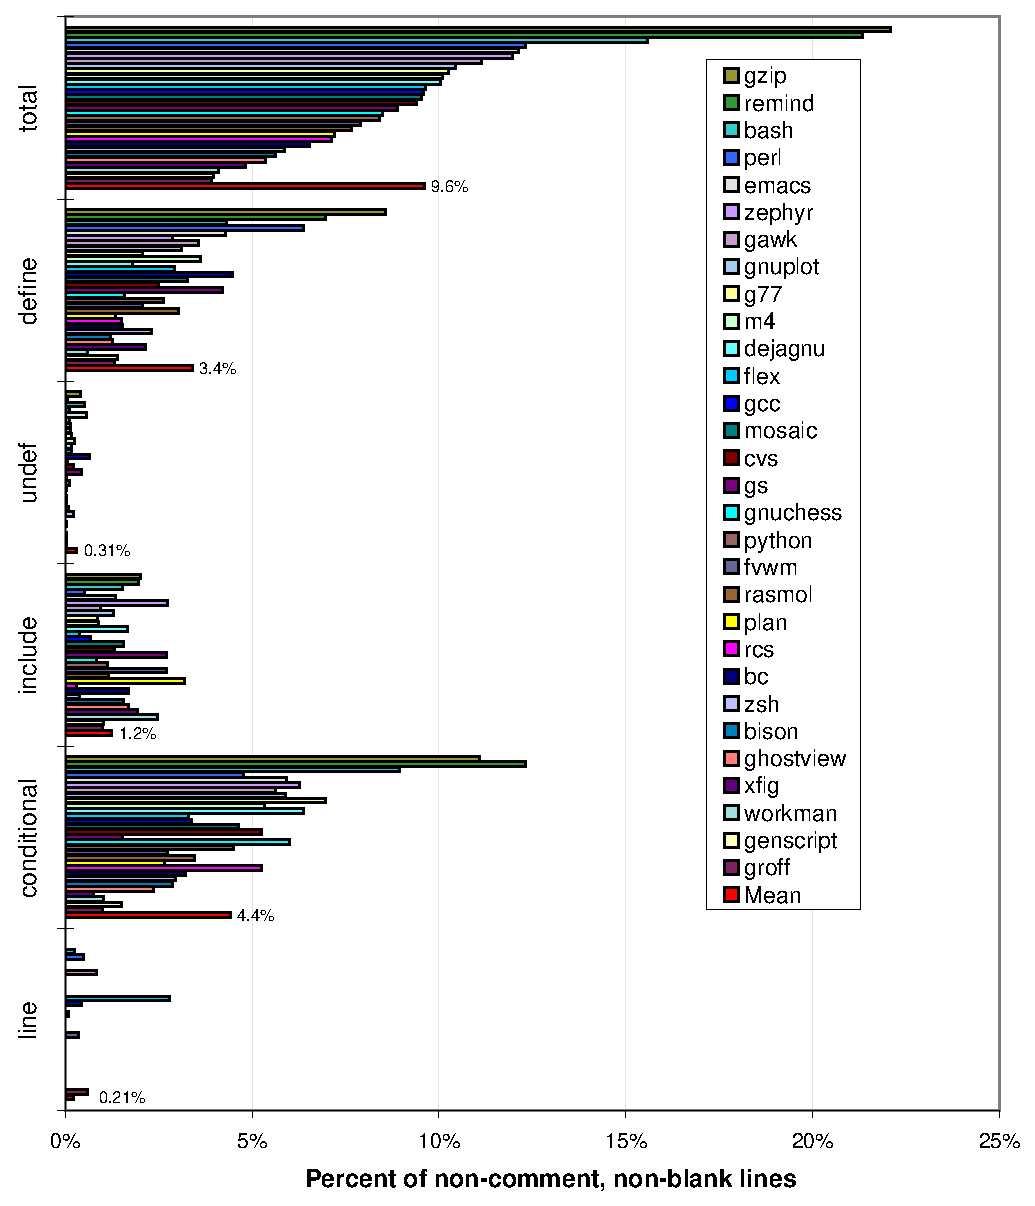
\epsfig{file=fig/directives-breakdown.eps,height=7.5in}}
\caption{Preprocessor directives as a fraction of non-comment,
  non-blank (NCNB) lines.}
\label{fig:directives-breakdown}
\end{figure}

The prevalence of preprocessor use makes understanding CPP constructs
crucial in any analysis of a program.  One in ten program lines is a
preprocessor directive rather than C code.  Across
packages, the percentage varies from less than 4\% to more than 22\%.
(These figures do not include the 28\% of lines which expand a macro or the
38\% of lines whose inclusion is controlled by {\tt \#if}; see
section~\ref{sec:dependence}.)

% \#if 46\%, \#define 35\%, \#include 13\%, \#undef 3\%, \#line 2\%

Conditional compilation directives account for just under half (46\%) of
the total directives in all packages, macro definitions comprise another
35\%, and file inclusion makes up most of the rest.  Packages are not very
uniform in their mix of preprocessor directives, however.  (If they were,
each group of bars in figure Figure~\ref{fig:directives-breakdown} would be
a scaled version of the top group.)  In particular, the prevalence of {\tt
\#include} is essentially independent of incidence of other directives.
The percentage of conditional directives varies from 16\% to 74\%, the
percentage of {\tt \#define} varies from 14\% to 52\%, and the percentage
of {\tt \#include}s varies from 4\% to 60\%.  This variation in usage
indicates that a tool for understanding Cpp cannot focus on just a subset
of directives.  


\subsection{{\tt \#line}, {\tt \#undef}, and other directives}

The definedness of a macro is often used as a boolean value.  However, {\tt
\#undef} is rarely used to set such macros to ``false''$\!$.  Most uses of
{\tt \#undef} immediately precede a definition of the just-undefined macro,
to avoid preprocessor warnings about incompatible macro redefinitions.

Every use of {\tt \#line} (in \pkg{bash}, \pkg{cvs}, \pkg{flex}, \pkg{fvwm},
\pkg{gawk}, \pkg{gcc}, \pkg{groff}, and \pkg{perl}) appears in lex or yacc
output that enables packages to build on systems lacking lex, yacc, or
their equivalents.  For instance, \pkg{flex} uses itself to parse its
input, but also includes an already-processed version of its input
specification (that is, C code corresponding to a {\tt .l} file) for
bootstrapping.

% , as are ``other'' directives (such as ).  
% as well as user-defined ones like {\tt \#module}

Rarely-appearing directives such as {\tt \#pragma}, {\tt \#assert}, and
{\tt \#ident}, and unrecognized directives, are omitted from
figure~\ref{fig:directives-breakdown}.  Among the packages we studied,
these directives account for .017\% of directives, or one in six thousand.
Their only significant user is \pkg{g77}, which contains 154 uses of {\tt
\#error} (representing 1.5\% of its preprocessor directives and 0.16\% of
its NCNB lines) to check for incompatible preprocessor flags.  We ignore
the null command (``{\tt \#}'' followed by only whitespace), which produces
no output.


\subsection{Packages with heavy preprocessor use}

The \pkg{gzip}, \pkg{remind}, and \pkg{bash} packages deserve
special attention for their heavy preprocessor usage\,---\,22\%, 21\%, and
16\%, respectively.

\pkg{gzip} {\tt \#define}s disproportionately many macros as literals and
uses them as arguments to system calls, enumerated values, directory
components, and more.  These macros act like {\tt const} variables and are
evidence of good programming style.  \pkg{gzip} also contains many
conditional compilation directives, since low-level file operations (such
as setting creation time and access control bits, accessing directories,
and so forth) are done differently on different systems.

\pkg{remind} supports speakers of ten different languages (and various
character sets) by using {\tt \#define}d constants for basically all user
output.  It also contains disproportionately many conditional compilation
directives; over half of these test the definedness of \verb|HAVE_PROTO|,
in order to provide both K\&R and ANSI prototypes.

Like \pkg{gzip}, \pkg{bash} is portable across a large variety of
systems, but \pkg{bash} uses even more operating system services.
Ninety-seven percent of \pkg{bash}'s conditional compilation directives
test the definedness of a macro whose presence or absence is a boolean
flag indicating whether the current system supports a specific feature.
The presence or absence of a feature requires different (or sometimes
additional) system calls or other code.


\section{Macro definition bodies}

This section examines features of macro definitions that may complicate
understanding the containing program.  We report how many macro definitions
expand to a partial or unidentifiable syntactic entity, take advantage of
special Cpp features that lie outside the programming language, or contain
other error-prone constructs.  We then turn to multiple definitions of a
particular macro name.  Multiple definitions can complicate understanding,
even if they do effectively the same thing.  We report on incidence of
redefinitions and of differing redefinitions, especially redefinitions with
incompatible bodies.

[[Punchline/summary goes here.]]


\subsection{Macro body categorization}

We categorized macro bodies into 28 categories, though for simplicity of
presentation, this paper coalesces these into ten higher-level categories.
We started with a set of categories that we expected to occur frequently
(similar to other macro
taxonomies~\cite{Stroustrup-DesignEvolution,Carroll95}), then iteratively
refined them to break up overbroad categories or add unforeseen ones.

Figure~\ref{fig:categorization} reports, for each package, how many
definitions create an expansion which falls in each category.  Macros which
act like C language constructs\,---\,such as variables or
functions\,---\,are easiest to understand and to translate into the
programming language, so there is reason to be optimistic for the 70\% of
macros whose bodies are expressions and the 6\% that are statements.  Other
macros, especially those which do not expand to a complete syntactic
construct, are more problematic.


The ten categories are as follows.  The examples are chosen for clarity
and brevity from the packages studied.

% Where does this go?
% There's no pattern, again.  (Nor is there a pattern by package size
% or by type of application.)

% The following isn't quite enough to get the columns lined up in this table.
% \newcolumntype{d}{D{.}{.}{2}}
% \begin{tabular}{|l|d|d|d|d|d|d|d|}\hline
\begin{figure}
% {\small
%   \setlength{\tabcolsep}{.25em}
%   \centerline{\begin{tabular}{|l|c|c|c|c|c|c|c|}\hline
Package & Null define & Literal & Expression & Statement & Stringization and pasting & Other syntatic macros & Failed classification\\\hline
Python & 176 & 510 & 865 & 50 & 5 & 62 & 21\\\hline
bash & 717 & 679 & 637 & 3 & 3 & 62 & 30\\\hline
bc & 4 & 36 & 37 & 2 & 0 & 9 & 1\\\hline
bison & 4 & 64 & 32 & 0 & 0 & 2 & 0\\\hline
cvs & 106 & 683 & 530 & 58 & 0 & 69 & 116\\\hline
flex & 32 & 224 & 87 & 19 & 0 & 36 & 2\\\hline
fvwm & 48 & 748 & 122 & 11 & 0 & 27 & 1\\\hline
gawk & 49 & 243 & 391 & 11 & 0 & 59 & 23\\\hline
genscript & 8 & 71 & 39 & 0 & 0 & 9 & 0\\\hline
\hline
Total & 1144 & 3258 & 2740 & 154 & 8 & 335 & 194\\\hline
\end{tabular}\\\hline
}%
% }
\centerline{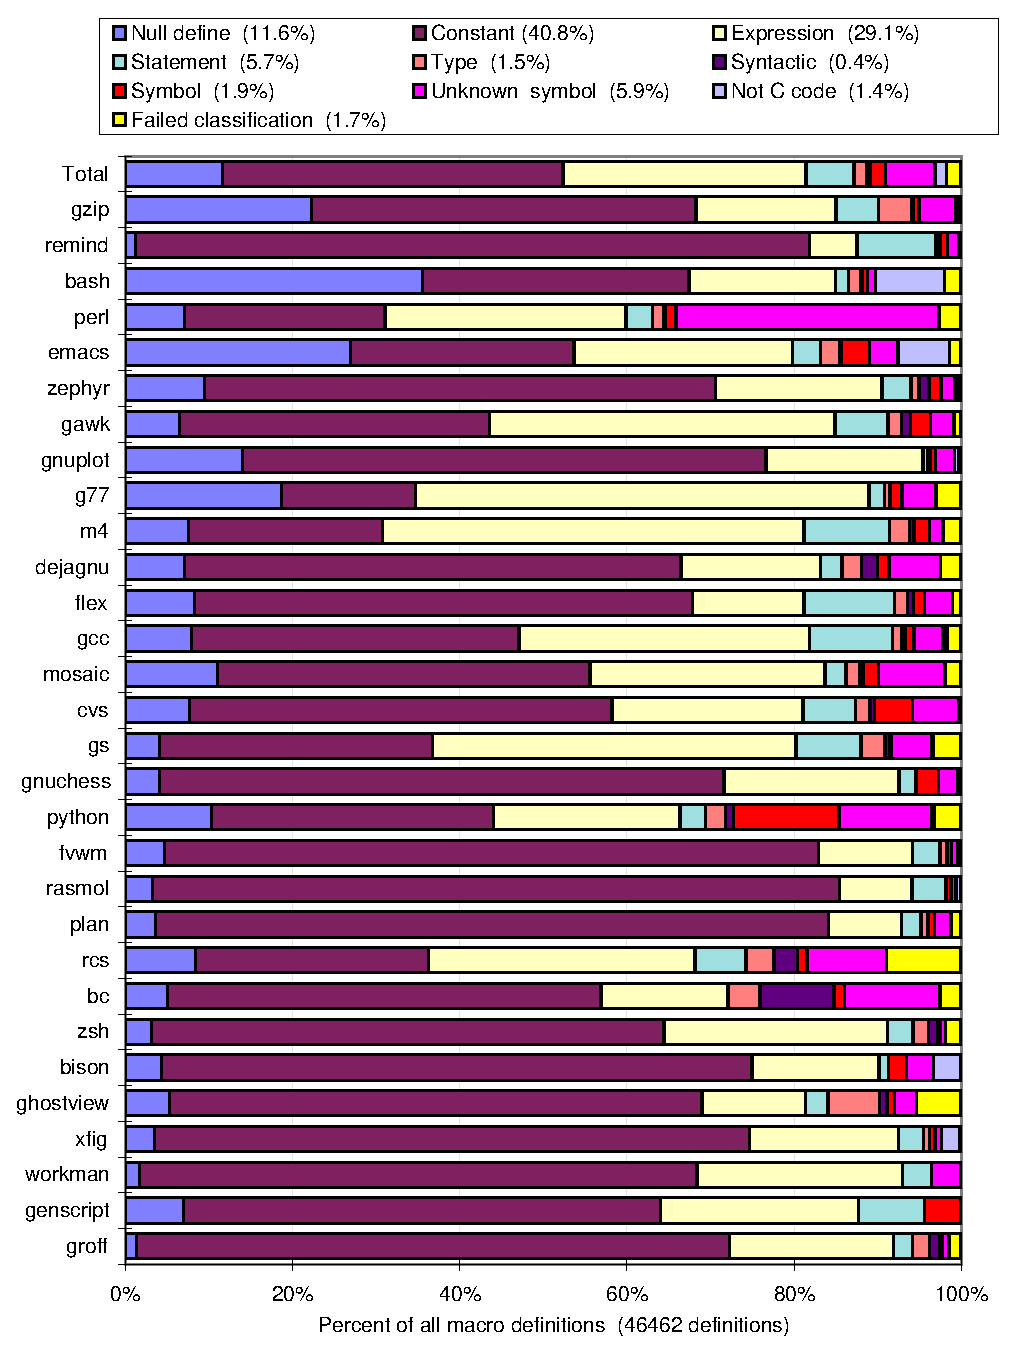
\epsfig{file=fig/def-categories.eps,height=6in}}
\caption{Categorization of macro definition bodies.  The legend numerically
  represents the information in the top row[[; the category names in the
  legend should be read across, by rows]].}
\label{fig:categorization}
\end{figure}


\label{sec:categorization}


{

\begin{description}
  \sloppy
  \emergencystretch=2em

%%  mcat_NULL: 5391
%%    100%  null_define (5391)
% @mcat_NULL = qw( catNULL_DEFINE );
\item[Null define]  The {\tt \#define} gives only an
  identifier name but no macro body, as in {\tt \#define
  \verb|HAVE_PROTO|}\@.  Such macros appear frequently in Cpp
directives (such as {\tt \#ifdef}), where they are used as boolean
variables by the preprocessor.  In code, they often represent optional
syntax.  For instance,
macro {\tt private} may expand either to {\tt static} or to nothing,
depending on whether a debugging mode is set.

%%  mcat_CONSTANT: 18971
%%    0.00%  constant (0)
%%    97%  literal (18426)
%%    2.9%  some_constant (545)
% @mcat_CONSTANT = qw( catCONSTANT catLITERAL catSOME_CONSTANT );
\item[Constant] The macro body is either a literal (97\% of this category)
  or an operator applied to constant values (3\% of this category).
  These macros act like {\tt const} variables. 
  For instance, {\tt \#define NULL 0}, {\tt \#define \verb|ARG_MAX|
  131072}, and {\tt \#define ETCHOSTS "/etc/hosts"} define literals, while
{\tt \#define \verb|RE_DUP_MAX| ((1<<15)-1)} and {\tt
\#define \verb|RED_COLS| (1 << \verb|RED_BITS|)} (where \verb|RED_BITS| is
a constant, possibly a literal) define constants.  This category includes
both macros whose value is invariant across all configurations of the
package and those which depend on other compile-time values.  

%%  mcat_NONCONSTANT_EXPRESSION: 13529
%%    100%  expression (13529)
% @mcat_NONCONSTANT_EXPRESSION = qw( catEXP );
\item[Expression]  The macro body is an expression, as in {\tt \#define
  sigmask(x) (1 << ((x)-1))} or {\tt \#define mtime mailfiles[i]->\verb|mod_time|}.
Such a macro acts like a function which returns a value (though the
macro need not take any arguments, so may look syntactically unlike a function).
The expression might have a single constant value everywhere (the usual
case for expression macros without arguments, most of which are classified
as constants, above) or might have a different value on each use (the usual
case for expression macros with arguments).

%%  mcat_STATEMENT: 2656
%%    47%  statement (1242)
%%    45%  semicolonless_statement (1197)
%%    1.5%  partial_statement (40)
%%    3.0%  statements (79)
%%    3.5%  semicolonless_statements (94)
%%    0.15%  partial_statements (4)
% @mcat_STATEMENT = qw( catSTATEMENT catSTATEMENT_SANS_SEMI catPARTIAL_STATEMENT
%                        catSTATEMENTS catSTATEMENTS_SANS_SEMI catPARTIAL_STATEMENTS );
% These aren't great examples (not from actual code); but so be it, as the
% actual examples are *very* long.
\item[Statement]  The macro body is a complete statement such as
  ``{\tt x = 3;}'', ``{\tt if (s) free(s);}'' or ``{\tt \verb|{| int x =
    y*y; printf("\%d", x); \verb|}|}''.  Such a macro is like a function
    returning {\tt void}, except that uses should not be followed by a
    semicolon (see section on macro lint: \ref{sec:lint}).
    
    To reduce the number of categories in this presentation, the statement
    categogry aggregates single statements (comprising 47\% of the category),
    statements missing their final semicolon (as in {\tt \#define QUIT if
    (\verb|interrupt_state|) \verb|throw_to_top_level|()}; these account
  for 45\%), multiple statements (3.0\%), multiple statements where the
  last one is missing its final semicolon (3.5\%), and partial statements
  (as in {\tt \#define ASSERT(p) if (!(p)) botch(\verb|__STRING|(p));
  else}; these are the final less than 2\%).

%%  mcat_TYPE: 697
%%    82%  type (569)
%%    0.00%  partial_type (0)
%%    3.3%  declaration (23)
%%    15%  semicolonless_declaration (105)
% @mcat_TYPE = qw( catTYPE catPARTIAL_TYPE catDECLARATION catDECLARATION_SANS_SEMI);
% #my @mcat_DECLARATION = qw( catDECLARATION catDECLARATION_SANS_SEMI );
% #folded DECLARATION into the above, TYPE
% The DECLARATION ones are quite rare.
\item[Type-related] 
  These macros expand to a type or partial type (such as a storage class),
  or expand to a declaration (possibly missing its terminating semicolon).
  [[Not all such are caught in the ``type'' category; some get classified
  as ``multiple symbols''.]]  Examples include {\tt \#define \verb|__ptr_t|
  void *}, {\tt \#define \verb|__INLINE| extern inline}, {\tt \#define
private static}, {\tt \#define \verb|FLOAT_ARG_TYPE| union \verb|flt_or_int|}, and {\tt
\#define CMPtype SItype}.  As a result, these macros may be tricky to
understand, and cannot be eliminated via straightforward translation
(though C++ templates may provide some hope).



%%  mcat_SYNTAX: 189
%%    18%  mismatched_entities (34)
%%    82%  punctuation (155)
% This includes ( catUNBALANCED catPUNCTUATION )
\item[Syntactic]  The macro body is either punctuation (as in
  {\tt \#define AND ;}, making up 82\% of this category) or contains
  unbalanced parentheses, braces, or brackets.  The latter are often used
  to create a block and perform actions that must occur at its beginning
  and end, as for \verb|BEGIN_GC_PROTECT| and \verb|END_GC_PROTECT|.
  
  Like stringization and pasting, these macros make essential use of the
  unique features of the preprocessor.


%%  mcat_SYMBOL: 870
%%    1.7%  reserved_word (15)
%%    94%  function_name (820)
%%    4.0%  symbols (35)
% @mcat_SYMBOL = qw( catRESERVED_WORD catFUNCTION_NAME catSYMBOLS);
\item[Symbols]
  The macro body is a single identifier that is either a function name
  (94\% of this category) or a reserved word (2\%, much of it uses of
  variable names which are reserved in another dialect).  A macro body
  which is a macro name inherits that macro's classification rather than
  appearing here.
  
  In this paper's presentation, a macro is also placed in this category if
  it expands to a space-separated sequence of symbols which cannot be
  positively identified as a partial declaration or other construct.  This
  accounts for the other 4\% of this category and is a failed
  categorization of sorts, but occurs frequently enough to deserve special
  notice.

  We are concerned with how it {\em could} be used, not just how it {\em
  happens} to be used.  That's why we can't take the easy out.  But it
  would be interesting to look at uses, which would let us infer the {\em
  intended} use (if not all {\em possible} uses).  We are actively pursing
  this line of research.

  Multiple adjacent identifiers\,---\,as in
  {\tt \#define EXFUN(name, proto) name proto} and {\tt \#define
  \verb|DO_OP|(OP,a,b) (a OP b)}\,---\,caused many failures of our
  classification heuristics.  Of the 1025 classification failures in the
  {\numpackages} packages, 496 were caused by a single definition in
  \pkg{gnuplot}, {\tt \#define CUR \verb|cur_term->type.|} (the period is
  part of the expansion), and uses of that macro, as in {\tt \#define
  \verb|acs_plus| CUR Strings[408]}.  Four packages\,---\,\pkg{bison},
  \pkg{gnuchess}, \pkg{remind}, and \pkg{workman}\,---\,had no macro
  classification failures.  These packages contain 93, 297, 932, and 58 macro
  definitions, respectively.




%%  mcat_SYMBOL_UNKNOWN: 2765
%%    100%  unknown_symbol (2765)
% @mcat_SYMBOL_UNKNOWN = qw( catSYMBOL_UNKNOWN );
\item[Unknown symbol]
  The macro expands to a single symbol which is not defined in the package
  or in any library header files included by the package.  The symbol may
  be defined by compiler command lines or may only be meaningful with a
  particular architecure, system, or library for which we did not have
  header files available (and used only inside an appropriate conditional
  compilation guard).  If the macro name has another definition which is
  not an unknown symbol, then we can safely assume that the inaccessible
  definition has similar characteristics.

  Unknown symbols can also be variables or functions that we failed to
  parse.  We use an approximate parsing technique that can succeed where an
  exact parse would no (as for unsyntactic code or entities broken by
  preprocessor directives), but somesimes fail to recognize all
  declarations and definitions.


%%  mcat_NON_C_CODE: 639
%%    90%  command_line_arguments (574)
%%    10%  assembly_code (65)
% @mcat_NON_C_CODE = qw( catCOMMAND_LINE catASSEMBLY_CODE );
\item[Not C code]  The predominant use of such macros is for 
  filenames and operating system command lines (together, 90\% of this
  category) and assembly code (the remaining 10\%).  The former usually
  appear in a file which is used by the preprocessor both when run over
  code and Makefiles.  We use conservative heuristics to determine when a
  line belongs in this category\,---\,after all, {\tt \#define
  \verb|SYSDEP_CFLAGS| -43 -w} creates a perfectly valid C
  expression\,---\,so we misclassify some such macros.  (See the ``expression
  plus not C code'' line at 0.14\% in figure~\ref{fig:subset-categories}.)
  
  The assembly code component includes only macros whose expansion is
  assembly code (as opposed to expressions and statements which happen to
  contain snippets of assembly code) makes up 10\% of this category.
  
  (We see those macros because: 1. we process all the .h files, and 2. some
  files are used for preprocessing both code and Makefiles, etc.  This
  latter use is problematic in itself, because by definition CPP is
  supposed to get a syntactic C program; it should err if what's between
  single quotes isn't a legal character constant, etc.  But many
  implementations don't perform any such checks.)


%%  mcat_FAILURE: 802
%%    0.00%  uncategorized (0)
%%    7.9%  being_categorized (63)
%%    10%  never_defined (82)
%%    78%  failed_categorization (628)
%%    3.6%  multiply_categorized (29)
% @mcat_FAILURE = qw( catNOT_YET catIN_PROCESS catNO_DEF catFAILURE catMULTIPLE );
\item[Failed classification]

Varargs.
Uses of pasting.
Complicated operating system command lines or flags.
Uses of other macros which have multiple definitions, or complicated
        definitions (we don't try to expand the latter, though probably we should).
Partial statements (e.g., case labels, parts of structure declarations), Partial expressions.
Passing in operators, as in "cmp".
Use of non-portable extensions.
C++ code.
Tricky declaration argument stuff:  ARGS2(t,a,u,b) (a,b) t a; u b;
JMESSAGE(code,string) string ,



  [[This needs to be rewritten, probably.]]
  [[Need to discuss why definitions fail, and give examples.]]

  Some of these are just limitations of our parser.

  The classifications are heuristic.  Maybe we could do better by fully
  expanding.

  
  Our tool failed to categorize less than 2\% of the 46462 definitions
  [[plus a small number of ``multiple symbols'']]; performing even a single
  level of macro expansion in bodies would make most of the latter
  failures, and many of the former ones, categorizable.  Other
  straightforward improvements include making a second pass after an
  initial categorization and using dependence information to determine
  which definitions can be active at an invocation site.  We have not
  pursued these enhancements, primarily because our tool is already
  accurate enough for our purposes.


% and illegal identifier
%   names ({\tt \#define \verb|FAT$C_VFC| 3} for VMS compilation), tokens %$HACK
%   ({\tt \#define \verb|LIB_PATH| /usr/ucblib}), and constants ({\tt 1ULL} for
%   {\tt unsigned long long})

%   \pkg{gnuplot}
%   contains only 13 other failures, ghostscript has 130, and no other
%   package stands out with many.

% half appeared in \pkg{gnuplot};
% \pkg{gnuplot}, cvs, and \pkg{groff} accounted for over 75\% of the failures, many of
% which could be eliminated by slightly relaxing the parsing rules.
\end{description}

%%% Local Variables: 
%%% mode: latex
%%% TeX-master: "emp-use-2"
%%% End: 
}

Figure~\ref{fig:categorization} shows the percentage of macros that fit
into these categories for each package.  Overall, 70\% of macro bodies are
expressions\,---\,mostly constants.



%In anticipation of the translator tool, the analysis tool infers
%types, using techniques similar to those of Siff and Reps~\cite{Siff-fse96}
%and O'Callahan and Jackson~\cite{OCallahan-icse97}.  Our use of the
%type information is in the early stages, however, and we do not report
%on the preliminary results in this paper.

% [FIX: Benefits even from simple literal constant conversion -- exposes
% symbolic information to the debugger]

%[FIX: Should this also include Mike's manual breakdown into categories
%for gzip.]



\subsection{Extra-linguistic capabilities}
\label{sec:extralinguistic}

The C preprocessor has capabilities outside the C programming language;
indeed, this is a primary motivation for using Cpp.  Such constructs
can present special challenges to program understanding, and especially to
elimination of the preprocessor by translation into C or C++.  This section
presents a list of such features and evaluates their frequency of
appearance, both individually and in combination,  in our test suite.

[[Since types are not first-class in C, they may not be passed to functions
or returned as results.]]

\begin{figure}
  {\small\centerline{
%\usepackage{graphics}
%\newcommand{\black}{\ensuremath{\blacksquare}}
\newcommand{\black}{\vrule height5.5pt depth0.5pt width6pt}
{\small
\addtolength{\columnsep}{-.5\columnsep}
% The *{n}{c|} below creates n duplicate columns of that type (centered, here)
\begin{tabular}{|r|*{8}{c|}}\hline
\rotatebox{90}{\parbox{1in}{Percentage of~ \\ 27228 macro \\ definitions}~} &
\rotatebox{90}{Free variables~(12\%)~} &
\rotatebox{90}{Assignment~(6.4\%)~} &
\rotatebox{90}{Use macro as type~(3.3\%)~} &
\rotatebox{90}{Pass type as argument~(0.44\%)~} &
\rotatebox{90}{Use argument as type~(0.070\%)~} &
\rotatebox{90}{Pasting~(0.037\%)~} &
\rotatebox{90}{Stringization~(0.029\%)~} &
\rotatebox{90}{Self-referential~(0.026\%)~}
\\ \hline
8.7\% &\black& & & & & & & \\ \hline
3.1\% &\black&\black& & & & & & \\ \hline
3.0\% & &\black& & & & & & \\ \hline
3.0\% & & &\black& & & & & \\ \hline
0.35\% & & & &\black& & & & \\ \hline
0.12\% & &\black&\black& & & & & \\ \hline
0.095\% &\black& &\black& & & & & \\ \hline
0.073\% &\black& & &\black& & & & \\ \hline
0.033\% & & & & &\black& & & \\ \hline
0.029\% &\black&\black&\black& & & & & \\ \hline
0.018\% & &\black&\black& &\black& & & \\ \hline
0.018\% & & & & & &\black& & \\ \hline
0.018\% & & & & & & &\black& \\ \hline
0.015\% &\black&\black& & & &\black& & \\ \hline
0.015\% &\black&\black& &\black& & & & \\ \hline
0.0073\% & &\black&\black& &\black& &\black& \\ \hline
0.0073\% & & & & & & & &\black\\ \hline
0.0073\% & &\black&\black& & & & &\black\\ \hline
0.0073\% & & &\black& &\black& & & \\ \hline
0.0073\% & &\black& & & & & &\black\\ \hline
0.0037\% & &\black& &\black& & & & \\ \hline
0.0037\% &\black& & & &\black& & & \\ \hline
0.0037\% &\black&\black& & & &\black&\black& \\ \hline
0.0037\% & & &\black& & & & &\black\\ \hline

\end{tabular}}
}}
  
  \caption{This figure indicates the occurrence, both singly and in
  combination, of the extra-linguistic capabilities of the C preprocessor
  listed in section~\ref{desc:properties}.  The features are listed across
  the top, along with the percentage of macro definitions exploiting each.
  Each row of the table reports the percentage of all macro definitions
  that exploit exactly a particular combination of the capabilities,
  indicated by black dots.  For instance, 0.093\% of all macro
  definitions both perform assignment and use the result of a macro
  invocation as a type, but use none of the other extra-linguistic features
  listed.  This table reports all macros using an extra-linguistic feature;
  the last several lines represent just one macro definition.}
  \label{fig:subset-properties}
\end{figure}

{\label{desc:properties}

\begin{description}
\item[Free variables]\label{page:freevar}
  The macro body uses as a subexpression (that is, applies an operator or
  function to) a symbol which is not a formal argument, a variable defined
  in the macro body, or a function, macro, typedef, or reserved word.  Such
  symbols are typically local or global variables.  Uses of global
  variables are generally innocuous; uses of local variables (in which the
  local definition in scope at the point of use captures the free variable
  in the macro body) can be used to achieve dynamic scoping, which C does
  not directly support.  We did not separately analyze global and local
  free variables.

\item[Assignment]
  The macro body side-effects state via assignment (of the form {\tt =},
  {\tt {\em op}=}, {\tt -{}-}, or {\tt ++}).  We did not look for calls to
  functions or macros that might have side effect, nor did we discount side
  effects to variables local to the macro body.  
  
  Assignment is not extra-linguistic per se, but macros containing
  assignment operators have potentially unexpected results (doubly so for
  those with no arguments, whose invocations look like variable uses, not
  function calls), some of which lie outside the scope of C\@.  A macro
  argument that is assigned to is similar to a pass-by-reference function
  argument and need only be noted in the macro's documentation.  A macro
  that assigns a global variable also presents no difficulties in
  understanding or translation into a C++ inline function.  Assignment to
  other variables free in the macro body demands that such a variable exist
  wherever the macro is invoked, and assigns to different variables at
  different invocations.  Such a macro implements a restricted form of
  dynamic scoping by capturing the instance of a variable visible at the
  point of macro invocation.

\item[Use macro as type]
  In this macro's body, the result of another macro invocation is used as a
  type\,---\,for instance, in a declaration or a type cast.  C cannot
  simulate this behavior, because its types are not first class; they may
  not be passed to functions, returned as results, or otherwise
  manipulated.

\item[Pass type as argument]
  In this macro's body, a literal type is passed to another macro, as in
  {\tt \#define PTRBITS \verb|__BITS|(char*)}.  Like using a macro result
  as a type, this is impossible in C\@.

\item[Pasting]\label{def:pasting}
  The body uses symbol pasting ({\tt \#\#}), which treats its arguments not
  as tokens but as strings, constructing a new token out of their
  concatenation, as in {\tt \#define \verb|_SIZEOF|(x) \verb|sz_|\#\#x},
  after which the macro invocation {\tt \verb|_SIZEOF|(int)} expands to the
  symbol {\tt sz_int}.  The resulting symbol might appear literally, or
  only as a pasted symbol, at its other uses.  Since pasting is often
  abstracted out into a separate macro\,---\,such as {\tt \#define
  \verb|__CONCAT|(x,y) x \#\# y}\,---\,the incidence of pasting is higher
than the direct uses reflected by this statistic.

\item[Use argument as type]
  This macro uses one of its arguments as a type.  Not all uses can be
  unambiguously identified lexically.  For instance, the macro 
  {\tt \#define \verb|MAKE_DECL|(type, name) type name;}
  is not identified as necessarily using its first argument as a type, for
  it might be invoked as {\tt \verb|MAKE_DECL|(printf, ("hello
  world\verb|\|n"))} or as {\tt \verb|MAKE_DECL|(x =, y+z)}.
  Like using a macro result
  as a type, this is impossible in C\@.

\item[Self-referential]
  The body refers to its own name, as in {\tt \#define LBIT vcat(LBIT)}.
  This feature is used when building a wrapper around an existing function
  or variable.  Since the ISO C preprocessor performs only one level of
  expansion on such recursively defined macros,\footnote{Pre-ANSI
    implementations were permitted to loop forever when expanding
    self-referential macros.} the expanded macro contains a reference to
  the original name.

\item[Stringization]
  The body uses argument stringization ({\tt \#}), which replaces its
  argument (a preprocessor symbol) by its contents as a C string.  After
  {\tt \#define FOO BAR BAZ}, the expression {\tt \#FOO} expands to {\tt
  "BAR~BAZ"}.  Examples using stringization include
\begin{verbatim}
    #define spam1(OP,DOC) {#OP, OP, 1, DOC},
    #define REG(xx) register long int xx asm (#xx)
\end{verbatim}
  No C or C++ language mechanism can replace such macros.  This feature is
  particularly useful in debugging, in order to print or record the exact
  operations being performed.

\end{description}


%%% Local Variables: 
%%% mode: latex
%%% TeX-master: "emp-use-2"
%%% End: 
}


The expected, specifically supported extra-linguistic features
(stringization, pasting) is neither the most prevalent nor the hardest to
comprehend:  it's the other uses based on the lack of structure in inputs
and outputs (both mere token streams), which enables arbitrary
transformations that programmers exploit in many ways.

  That only [[0.2\%]] of macros exploit
stringization or pasting, the only truly extra-linguistic capabilities in
the C preprocessor, is encouraging.

        About one in six macros (16.8\%) falls into at least one category

        We show an exact breakdown by subsets because, if we report by
          property, the numbers don't add to 100\%: sometimes a macro has
          multiple properties.

        Not as much use of stringization, pasting as we anticipated -- we
          had been particularly worried about them.

        The uses of types are going to be problematic.

[[Move this earlier?]]
[[These numbers aren't right any more -- not 10\%.]]
One tenth of expression macros in our study use assignment operators, which
have potentially unexpected results.  A macro argument that is assigned to
is similar to a pass-by-reference function argument and need only be noted in the
macro's documentation.  A macro that assigns a global variable also
presents no difficulties in understanding or translation into a C++
inline function.
Assignment to a local variable that is free in the macro body, however,
demands that such a variable exist wherever the macro is invoked, and
assigns to different variables at different invocations.\footnote{By
  contrast, LCLint~\cite{Evans:LCLint} considers assignment to a macro
  argument dangerous but does not appear to check for assignments to local
  variables.} Such a macro implements a restricted form
of dynamic scoping by capturing the instance of a variable visible at
the point of macro invocation.


\subsection{CPP pitfalls:  macro lint}
\label{sec:lint}

We identified a number of potentially dangerous programming
constructs\,---\, those which are legal (syntactically valid) and may well
be intentional, but which also might cause a macro not to behave as
anticipated (and not to behave like an ordinary function).  Nearly one
fourth of all definitions triggered at least one such warning; and across
macro names, almost one fourth contain a definition which triggers a
warning.

Because it flags such errors, our tool can be used as a sort of macro
lint.  A more polished implementation would permit each type of warning to
be enabled and disabled individually.

\begin{figure}
  {\small\centerline{\begin{tabular}{|l|l|l|} \hline
any warning by name & 4944 & 23\% \\ 
any warning by def & 5768 & 22\% \\ 
unparenthesized formal uses & 2447 & 9.3\% \\ 
multiple formal uses & 2233 & 8.5\% \\ 
free variables & 2220 & 8.5\% \\ 
unparenthesized body & 1170 & 4.5\% \\ 
dangling semicolon & 535 & 2.0\% \\ 
side-effected formal & 333 & 1.3\% \\ 
swallows else & 245 & 0.93\% \\ 
inconsistent arity by name & 92 & 0.42\% \\ 
null body with args & 106 & 0.40\% \\ 
bad formal name & 19 & 0.072\% \\ 
\hline
\end{tabular}
}}
  
  \caption{Macro lint.}
  \label{fig:macro-lint}
\end{figure}

{
\begin{description}
\item[free variables]
  See page~\pageref{page:freevar} for a discussion of issues related to
  free variables.  We specifically check for side-effected formal arguments
  as well; see below.

\item[multiple formal uses]
        Some argument is used as an expression multiple times, so any side
        effects in the actual argument expression will occur multiple
        times.  
        Given a macro defined as
\begin{verbatim}
    #define EXP_CHAR(s) (s == '$' || s == '`' || s == CTLESC)
\end{verbatim}
        an invocation such as {\tt \verb|EXP_CHAR|(*p++)} increments the
        pointer by three locations rather than just one as intended (and as
        would occur were \verb|EXP_CHAR| a function).  Even if the argument
        has no side effects, as in \verb|EXP_CHAR|(peekc(stdin)), repeated
        evaluation may be unnecessarily expensive.
        
        Some C dialects provide an extension for declaring a local variable
        within an expression.  In GNU C~\cite{GCC}, this is achieved in the
        following manner:
\begin{verbatim}
    #define EXP_CHAR(s) ({ int _s = (s); (_s == '$' || _s == '`' || _s == CTLESC) })
\end{verbatim}

\item[unparenthesized formal uses]
        Some argument is used as a subexpression (i.e., is adjacent to an
        operator) without being enclosed in parentheses, so that precedence
        rules could result in an unanticipated computation being performed.
        For instance, in
\begin{alltt}
    #define DOUBLE(i) (2*i)
    \ldots\ DOUBLE(3+4) \ldots
\end{alltt}
        the macro invocation computes the value 10, not 14.
        This warning is suppressed when the argument is the entire body
        or is the last element of a comma-delimited list (which has 
        low precedence).

\item[unparenthesized body]
        The macro body is an expression which ought to be parenthesized to
        avoid precedence problems at the point of use.  For instance, in
\begin{alltt}
    #define DOUBLE(i) i+i
    \ldots\ 3*DOUBLE(4) \ldots
\end{alltt}
        the expression's value is 16 rather than 24.
        
        This warning is applicable only to macros that expand to an
        expression and is suppressed if the body is a single token or a
        function call (which has high precedence).

\item[doesn't swallow semicolon]\label{item:swallow-semicolon}
        The macro body takes arguments and expands into a statement or
        multiple statments.  Thus, its invocations look like function
        calls, but it cannot be legally used like a function call, as in
\begin{alltt}
    #define ABORT() kill(getpid(),SIGABRT);
    \ldots
    if (*p == 0)
      ABORT();
    else \ldots
\end{alltt}
        because {\tt ABORT();} expands to two statements (the second a null
        statement), which is unsyntactic between the {\tt if} condition and
        {\tt else}.

        Macros without arguments, such as {\tt \#define \verb|FORCE_TEXT|
        \verb|text_section|();}, suppress this warning on the theory that their
        odd syntax will remind the programmer not to add the usual semicolon.

        The solution to this problem is to wrap the macro body in
\begin{alltt}
             do \verb|{| \ldots\ \verb|}| while (0)
\end{alltt}
        which is a partial statement that requires a final semicolon.  To
        our surprise, we found few uses of this standard, widely-recommended
        construct but many error-prone uses of statement macros followed by
        semicolons.

\item[null body with arguments]
        The macro is a null define of the form {\tt \#define name(e)} 
        which might have been intended to be {\tt \#define name (e)}.
        An empty comment is the idiomatic technique for indicating that the
        null definition is not a programming error, so a comment where the macro
        body would be suppresses this error, as in
\begin{verbatim}
    #define __attribute__(Spec) /* empty */
    #define ReleaseProc16(cbp) /* */
    #define __inline /* No inline functions.  */
    #define inline /**/
\end{verbatim}

\item[side-effected formal]
        A formal argument is side-effected.  This is erroneous if the
        argument is not an lvalue.  A similar constraint applies to
        reference parameters in C++, which can model such macro arguments.

\item[inconsistent arity]
        The macro name is defined multiple times with different arity; for example,
\begin{verbatim}
    #define ISFUNC 0
    #define ISFUNC(s, o) ((s[o + 1] == '(')  && (s[o + 2] == ')'))
\end{verbatim}
        This may indicate either a genuine bug or a macro name used for
        different purposes in different parts of a package, in which case
        the programmer must take care that the two are never simultaneously
        active (lest one override the other).  The latter situation may be
        caught by Cpp's redefinition warnings, if the macro name is not
        subjected to {\tt \#undef} before the second definition.

\item[swallows else]
        The macro, which ends with an {\tt else}-less {\tt if} statement,
        swallows any {\tt else} clause that follows it.  For instance, after
\begin{verbatim}
    #define TAINT_ENV() if (tainting) taint_env()
    #define merge_(a,b) if (TM_DEFINED (b)) (a) = (b);
\end{verbatim}
        a use like
\begin{alltt}
    if ({\em condition})
      TAINT_ENV();
    else \ldots
\end{alltt}
        results in the {\tt else} clause being executed not if  the
        condition is false, but if it is true (and {\tt tainting} is also
        true).
        
        This problem results from a potentially incomplete statement (though
        an {\tt if} statement doesn't require an {\tt else} clause) which
        may be attached to some following information.  It is the mirror of
        the ``doesn't swallow semicolon'' problem listed above which
        resulted from a too-complete statement which failed to be
        associated with a textually subsequent token.  The solution is
        similar: either add an else clause with an empty statement, as in
        {\tt \#define ASSERT(p) if (!(p)) botch(\verb|__STRING|(p)); else}, or
        wrap statements in {\tt \verb|{| \ldots\ \verb|}|} and wrap partial
        statements in {\tt do \verb|{| {\rm \ldots}\ \verb|}| while (0)}.

\item[bad formal name]
        The formal name is not a valid identifier or is a reserved word
        (possibly in another dialect of C).
\begin{verbatim}
#define CR_FASTER(new, cur) (((new) + 1) < ((cur) - (new)))
\end{verbatim}
        This presents no difficulty to Cpp, but a programmer reading the
        body (especially a more complicated one) may become confused.

\end{description}



%%% Local Variables: 
%%% mode: latex-mode
%%% TeX-master: "emp-use-2"
%%% End: 
}




The lint tables exclude all non-C-code; also all definitions not in the package.

        We didn't examine every use.  Besides, the point isn't just the
          current uses, but also future uses:  we want these to be easy for
          programmers to use.

        We also discovered a number of files which begin or end inside a
          brace scope or an {\tt \#if} scope.  Some of these were intentional, while
          others are bugs (such as, in one case, a failure to close a /* */
          style comment) which were apparently not discovered because testing
          did not build the package under all possible circumstances.

          Use of old /**/-style pasting.

        Also warnings for unexpected indentation and more.

        Also some bad constructs:
          {\tt \#undef \verb|GO_IF_INDEXABLE_BASE|(X, ADDR)}
          {\tt \#module}

\subsection{Multiple definitions}

Refer to figure~\ref{fig:freq-def-cat}.  Explain why the numbers in its
legend differ from those in figure~\ref{fig:categorization}.

        When classifying a name (as opposed to a definition), "failed
          classification" includes "two different defs fell into different
          categories".  (We could also get that even if a single
          definition, earlier, if it expands to just such a macro.)
          Explain how we combine two different categories into a single one.

        Not C code tends to be for the benefit of Makefiles; compilation
          lines, library filenames, and such tend to differ for each
          operating system.  

        Syntactic is parentheses, commas, semicolons, critical section
          delimiters, etc:  frequently-used.  [[That's irrelevant:  here I
          want to know why there are so many {\em definitions}.]]

        It stands to reason that "failed classification" has multiple
          definitions, because when determining the category for a macro
          name, we categorize each definition, and if any of them are
          either failures or have different categories, then the classification
          for the name is "failure".  (See section~\ref{sec:inconsistent}.)

        Few for unknown symbol, because if any def isn't unknown symbol,
          then neither is the entire macro.

        By package (not pictured):  most follow the "Mean" curve.

          Half of packages have no macros defined more than 14 times.

          Notable exceptions to the rule:
            \pkg{bc}:  all macros are defined either one or two times

            \pkg{remind}:  10\% of macros are defined between 11 and 15 times
                (none defined 16 or more); uses macros for all user output.
                
                The \pkg{remind} program uses macro definitions to provide
                localization support for ten different natural languages
                (and multiple character sets for some of them), accounting
                for its surprisingly large number of macros with many
                definitions.

            \pkg{gcc}: over 4\% of macros are defined more than 20 times.
                gcc goes 99.5\% at 50 definitions.
                i.e., 99.5\% of macro names are defined 50 or fewer times.
                1 macro, \verb|CPP_PREDEFINES|, is defined 181 times (and undefined
                  198 times).
                Many of these aren't C code.

        % \section{Frequency of macro definition and usage}
        \label{sec:usage}

        % The second question we asked was: where and how often are macros
        % defined and used in practice?  

        % \begin{figure}
        % {\small
        %   \setlength{\tabcolsep}{.25em}
        %   \centerline{\begin{tabular}{|l|c|c|c|c|c|c|c|c|c|c|c|c|}\hline
\#Defs & Python & bc & bison & cvs & flex & fvwm & g77 & gawk & genscript & ghostview & glibc & gnuchess\\\hline%\hline
1  & 71.86 & 53.25 & 63.21 & 34.60 & 42.42 & 55.21 & 83.45 & 40.37 & 75.19 & 50.35 & 19.46 & 67.10\\\hline
2  & 84.48 & 100.00 & 87.74 & 66.09 & 87.15 & 82.00 & 93.52 & 70.82 & 89.15 & 75.89 & 52.14 & 78.06\\\hline
3  & 89.93 & 100.00 & 87.74 & 78.31 & 90.23 & 89.24 & 95.83 & 79.82 & 89.15 & 90.78 & 68.57 & 89.68\\\hline
4  & 92.36 & 100.00 & 91.51 & 86.05 & 94.34 & 90.12 & 96.59 & 81.66 & 92.25 & 96.45 & 75.47 & 96.13\\\hline
5  & 94.18 & 100.00 & 91.51 & 87.78 & 95.63 & 90.67 & 96.83 & 82.24 & 92.25 & 100.00 & 79.95 & 96.13\\\hline
6  & 96.36 & 100.00 & 91.51 & 88.60 & 97.17 & 90.67 & 96.83 & 82.93 & 92.25 & 100.00 & 84.32 & 100.00\\\hline
7  & 96.79 & 100.00 & 91.51 & 89.57 & 97.17 & 92.97 & 98.18 & 82.93 & 92.25 & 100.00 & 86.58 & 100.00\\\hline
8  & 97.76 & 100.00 & 91.51 & 90.12 & 97.17 & 93.85 & 98.94 & 83.85 & 92.25 & 100.00 & 90.28 & 100.00\\\hline
9  & 98.30 & 100.00 & 100.00 & 90.12 & 97.17 & 94.84 & 98.94 & 85.93 & 92.25 & 100.00 & 91.16 & 100.00\\\hline
10+ & 100.00 & 100.00 & 100.00 & 100.00 & 100.00 & 100.00 & 100.00 & 100.00 & 100.00 & 100.00 & 100.00 & 100.00\\\hline
\multicolumn{12}{c}{} \\
\cline{0-11}
\#Defs & gnuplot & groff & gs & gzip & plan & rcs & remind & workman & xfig & zephyr & zsh\\\cline{0-11}\cline{0-11}
1  & 69.76 & 33.06 & 74.41 & 35.48 & 72.55 & 56.83 & 35.61 & 68.33 & 86.69 & 61.31 & 78.79\\\cline{0-11}
2  & 82.35 & 75.86 & 90.92 & 70.40 & 96.08 & 83.06 & 38.87 & 91.67 & 91.72 & 88.82 & 94.64\\\cline{0-11}
3  & 86.38 & 85.14 & 95.87 & 79.78 & 98.43 & 91.26 & 42.45 & 91.67 & 93.61 & 92.67 & 96.39\\\cline{0-11}
4  & 90.51 & 92.27 & 97.36 & 86.40 & 100.00 & 95.63 & 45.49 & 91.67 & 94.03 & 94.22 & 97.32\\\cline{0-11}
5  & 92.57 & 92.27 & 97.36 & 90.99 & 100.00 & 95.63 & 46.58 & 100.00 & 95.60 & 94.86 & 97.32\\\cline{0-11}
6  & 93.81 & 98.69 & 97.61 & 94.30 & 100.00 & 95.63 & 46.58 & 100.00 & 96.23 & 95.63 & 97.32\\\cline{0-11}
7  & 94.53 & 98.69 & 98.18 & 98.16 & 100.00 & 95.63 & 49.62 & 100.00 & 96.23 & 95.63 & 97.32\\\cline{0-11}
8  & 95.36 & 98.69 & 98.51 & 98.16 & 100.00 & 100.00 & 49.62 & 100.00 & 96.23 & 96.66 & 97.32\\\cline{0-11}
9  & 95.36 & 98.69 & 98.51 & 98.16 & 100.00 & 100.00 & 50.60 & 100.00 & 96.23 & 96.66 & 97.32\\\cline{0-11}
10+ & 100.00 & 100.00 & 100.00 & 100.00 & 100.00 & 100.00 & 100.00 & 100.00 & 100.00 & 100.00 & 100.00\\\cline{0-11}\cline{0-11}
\end{tabular}
% Local Variables: 
% mode: latex
% TeX-master: "paper"
% End: 
}%
        % }
        % \caption{Number of definitions per Cpp identifier.  The numbers in the
        %   table represent the percentage of identifiers which are defined a given
        %   number of times or fewer.  For example, \pkg{bison} contains 4 or fewer
        %   definitions for 91.51\% of all Cpp macros it defines, and no
        %   macro is defined 5, 6, 7, 8, or more than 9 times.}
        % \label{fig:define_count}
        % \end{figure}

        \begin{figure}
        \centerline{\epsfig{file=fig/cat-def-frequency.eps,height=7.2in}}
        \caption{Number of definitions per Cpp identifier, graphed as
          the percentage of identifiers that are defined a given number of times
          or fewer.  Overall, 96\% of macros were defined three or
          fewer times; the other 4\% of macros had four or more distinct
          definitions ({\tt \#define} directives).}
        \label{fig:freq-def-cat}
        \end{figure}


% \begin{figure}
% \centerline{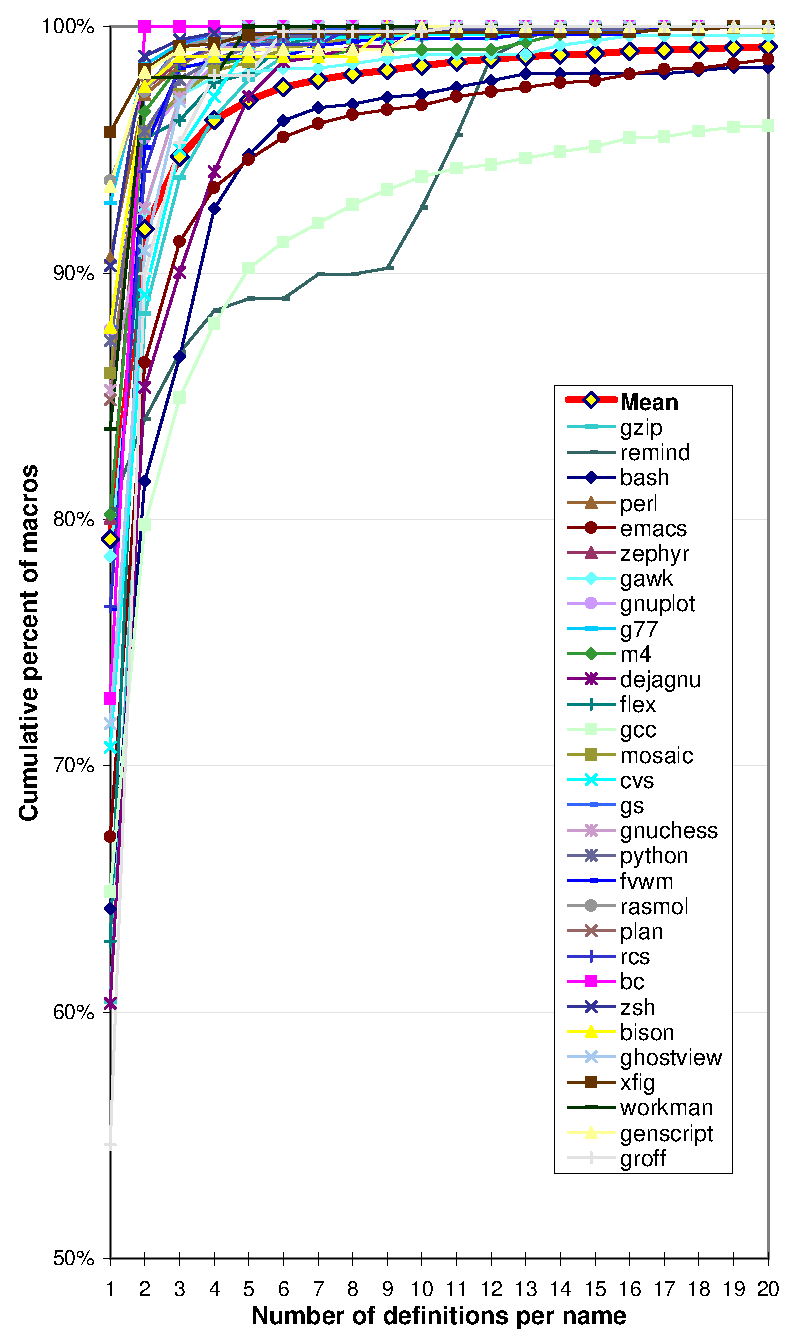
\epsfig{file=fig/def-frequency.eps,height=7.2in}}
% \caption{Number of definitions per Cpp identifier, graphed as
%   the percentage of identifiers that are defined a given number of times
%   or fewer.  Overall, 96\% of macros were defined three or
%   fewer times; the other 4\% of macros had four or more distinct
%   definitions ({\tt \#define} directives).  The outlier, for which 10\% of
%   macros are defined more than eight times, is the \pkg{remind}
%   package, which uses macros for all user output.}
% \label{fig:freq-def}
% \end{figure}

        
        No distinction is made between sequential redefinitions of a macro
        and multiple definitions that cannot take effect in a single
        configuration (say, because they appear in different branches of a
        Cpp conditional).  This is exactly the right thing!  Also, we merge
        together different definitions created by different files and
        either {\tt \#undef}ed or with different scopes.  That is, we have
        no notion of reaching definitions.
        

        [[Get new numbers, and repeat this analysis.]]  [[Check whether
        bash and dejagnu are even worht mentioning:  probably not.  but
        make the point about portability and libraries.]]
        In all but four packages, at least [[93\%]] of all macros are
        defined three or fewer times.  For \pkg{bash} and \pkg{dejagnu},
        such macros account for [[90\%]], largely because these packages
        are highly portable and also quite dependent on system libraries.


\subsection{Multiple distinct definitions}

\begin{figure}
  \centerline{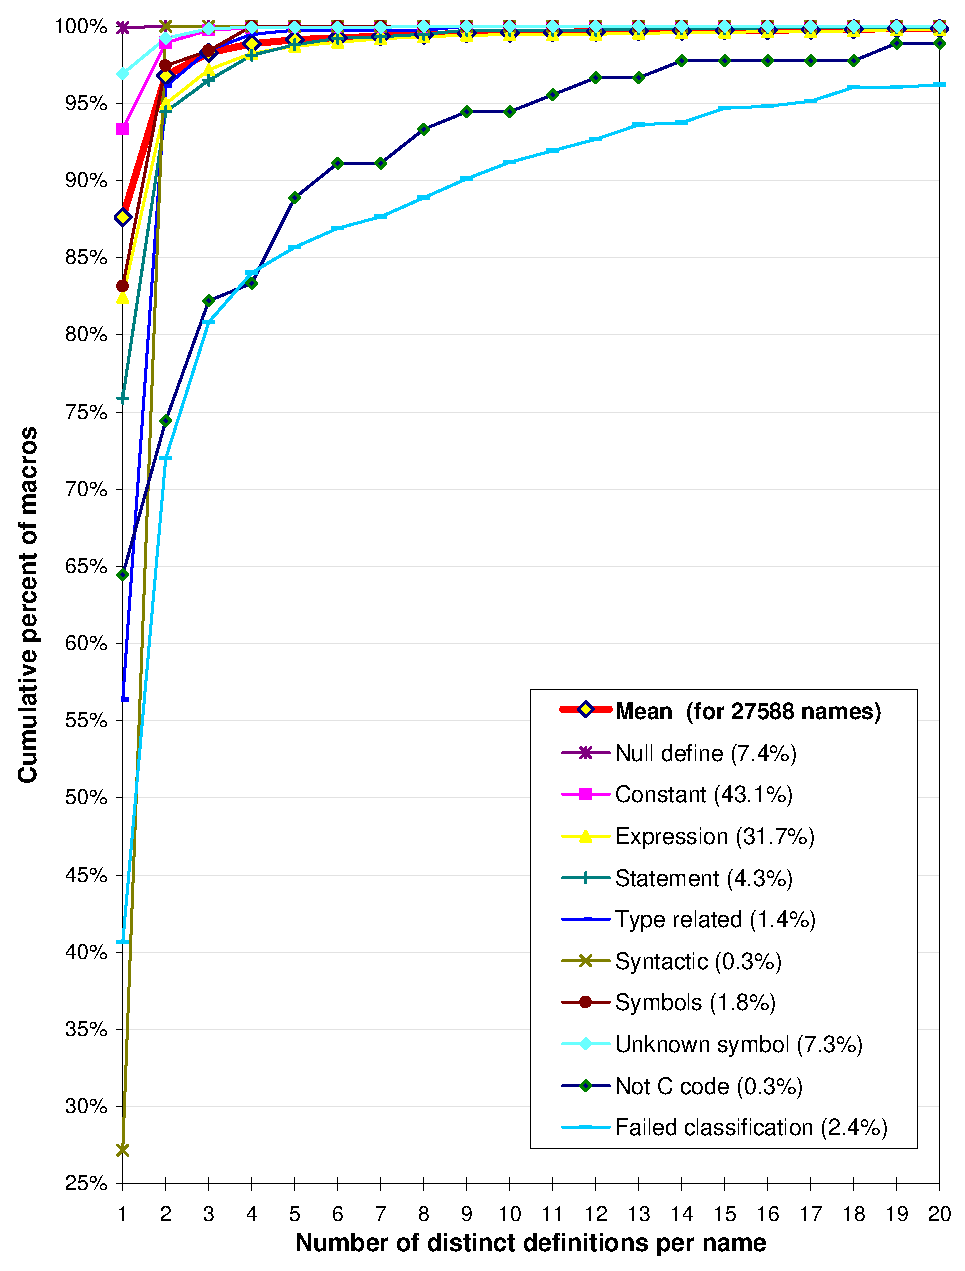
\epsfig{file=fig/cat-ddf-frequency.eps,height=7.2in}}
  \caption{Number of syntactically distinct definitions per Cpp identifier, graphed as
    the percentage of identifiers that are defined a given number of times
    or fewer.  [[Say something to help interpret it.]]  [[Give note
    about what's in legend, from text or previous figure?  Nah, just
    refer back, probably.]]}
  \label{fig:freq-ddf-cat}
\end{figure}
        
This uses a less strict rule than that used by CPP when determining whether
to issue a warning about redefinition.  We eliminate all comments and
whitespace, canonically rename all formal arguments, and compare all
character and string literals to be identical.  Thus, it is a lower bound
on the number of definitions with distinct abstract syntax trees, much as
the previous chart was an upper bound.

Even when two distinct definitions are identical, if they appear in
different locations then it is more likely that something used by that
definition has changed.  [[From chart not shown: we identify most of
\pkg{remind}'s definitions as non-distinct.]]

\subsection{Inconsistent definitions}
\label{sec:inconsistent}

Even among macros with multiple definitions, those different definitions
generally fall into the same, or compatible, categories.

\begin{itemize}
\item If the categories are the same, use that.

\item If one has no definition, is a null define, or is an unknown symbol, use
  the other.  [[This is fine for statement, type; but a bit iffy for
  expressions.]]

  [[If the macro name has another definition
  which is not an unknown symbol, then we can safely assume that the
  inaccessible definition has similar characteristics.]]

\item If one is a constant and the other is an expression, use expression.

\item If one is a symbol and the other is reserved word or type, choose the latter.

\item If one is statement-related, choose the other if it's the corresponding plural.
\item If one is statement-related, sans semicolon, choose the other if it's partial.
\end{itemize}

\begin{figure}
  {\small\centerline{
%\usepackage{graphics}
%\newcommand{\black}{\ensuremath{\blacksquare}}
\newcommand{\black}{\vrule height5.5pt depth0.5pt width6pt}
\begin{tabular}{|r|*{22}{c|}}\hline
\rotatebox{90}{\# Occurrences} &
\rotatebox{90}{failed categorization} &
\rotatebox{90}{null define} &
\rotatebox{90}{expression} &
\rotatebox{90}{expression with assignment} &
\rotatebox{90}{expression with free variables} &
\rotatebox{90}{literal} &
\rotatebox{90}{constant} &
\rotatebox{90}{some constant} &
\rotatebox{90}{has type argument} &
\rotatebox{90}{macro as function} &
\rotatebox{90}{macro as type} &
\rotatebox{90}{uses type argument} &
\rotatebox{90}{expands to type} &
\rotatebox{90}{expands to reserved word} &
\rotatebox{90}{statement} &
\rotatebox{90}{recursive} &
\rotatebox{90}{assembly code} &
\rotatebox{90}{syntax tokens} &
\rotatebox{90}{mismatched entities} &
\rotatebox{90}{token pasting} &
\rotatebox{90}{stringization}
\\\hline
    40\% & & & & & &\black& & & & & & & & & & & & & & &  \\\hline
    33\% & & &\black& & & & & & & & & & & & & & & & & &  \\\hline
   6.1\% & &\black& & & & & & & & & & & & & & & & & & &  \\\hline
   5.5\% &\black& & & & & & & & & & & & & & & & & & & &  \\\hline
   4.1\% & & & & & & & & & & & & & & &\black& & & & & &  \\\hline
   3.7\% & & & &\black& & & & & & & & & & & & & & & & &  \\\hline
   2.9\% & & & & & & & &\black& & & & & & & & & & & & &  \\\hline
  0.47\% & & & & & & & & & & & &\black& & & & & & & & &  \\\hline
  0.46\% & & & & & & & & & & & & &\black& & & & & & & &  \\\hline
  0.42\% & &\black& & & & & & & & & & & & &\black& & & & & &  \\\hline
  0.39\% & & & & & & & & & & & & & & & &\black& & & & &  \\\hline
  0.36\% & & &\black& & &\black& & & & & & & & & & & & & & &  \\\hline
  0.34\% & & & &\black& & & & & & & & & & &\black& & & & & &  \\\hline
  0.26\% & & & & & & & & & & &\black& & & & & & & & & &  \\\hline
  0.22\% & &\black&\black& & & & & & & & & & & & & & & & & &  \\\hline
  0.19\% & &\black& & & & & & & & & & &\black& & & & & & & &  \\\hline
  0.17\% & & &\black&\black& & & & & & & & & & & & & & & & &  \\\hline
  0.16\% & & &\black& & & & & & & & & & & &\black& & & & & &  \\\hline
  0.14\% &\black&\black& & & & & & & & & & & & & & & & & & &  \\\hline
  0.12\% & & & & & & & & & & & & & & & & & & &\black& &  \\\hline
  0.12\% & & &\black& & & & & & & & & & & & & & &\black& & &  \\\hline
  0.11\% & & &\black& & & & & & & & &\black& & & & & & & & &  \\\hline
   0.1\% &\black& &\black& & & & & & & & & & & & & & & & & &  \\\hline
 0.077\% &\black& & & & &\black& & & & & & & & & & & & & & &  \\\hline
 0.077\% & & & & & &\black& & & & & & & & &\black& & & & & &  \\\hline
 0.077\% & & & & & & & & & & & & & & & & & & & &\black&  \\\hline
 0.061\% & &\black& & & &\black& & & & & & & & & & & & & & &  \\\hline
 0.061\% & & & & & & & & & &\black& & & & & & & & & & &  \\\hline
 0.056\% &\black& & & & & & & & & & & & & &\black& & & & & &  \\\hline
 0.056\% & &\black& &\black& & & & & & & & & & & & & & & & &  \\\hline
 0.056\% & & & & & & & &\black& & & & & & & & & &\black& & &  \\\hline
 0.051\% & & & & & &\black& &\black& & & & & & & & & & & & &  \\\hline

\end{tabular}
}}
  \caption{Subset categorization of macros (not macro definitions).   Items
    less than [[one twentieth of a percent]] are omitted; such items appear
    fewer than [[ten]] times in the codebase.
    The arrows indicate macros for which the names would be classified
    as "failure" (2.4\% of macro names).}
  \label{fig:subset-categories}
\end{figure}

Two anomalies in arrows (ie, failing combinations) are due to the fact that
"statement" category should really be called "statement-related": it
includes full statements, statements missing a final semicolon, partial
statements, multiple statements, multiple statements plus a partial one.
\begin{itemize}
\item
  no arrow on one "expression + statement", at 1.1\%, because that was
  actually "expression + semicolonless statement" -- and an expression plus
  a semicolon also makes a statement.  For instance, the expressions could
  have been function calls.  The other, just below it, has slightly fewer
  occurrences (but both round to 1.1\%; it also contains "statement", which
  is incompatible with "expression").  Also compare the similar duplication
  at .26\% and .10\%.
\item
  arrow on just "statement" at .35\%: was actually "semicolonless
  statement, semicolonless statements, statement"
\end{itemize}





        Figure~\ref{fig:subset-categories} indicates that multiple definitions of a
        particular macro tend to be compatible.  It classifies macros rather than
        macro definitions.  Each macro is
        given a set of categorizations (corresponding to the categorizations of its
        definitions) and the incidence of each such is displayed.  For over [[97\%]] of
        macros, all of the macro's definitions are given compatible
        categorizations [[and for x\%, they're given exactly the same
        categorization in all cases]].

        [[What's going on with null define plus constant or expression??]]

\section{Uses}

\subsection{high usage}

        Give average uses per defined macro name (see new summary table).

        In the chart, a higher line indicates less use.

        Half of all macros are used two or fewer times (!).  12\% not used
          at all (!).

        Syntactic macros tend to be used far more often; also those
          expanding to a type.  These make sense, as they are
          frequently-used constructs 
          that permeate code (appear at every definition, for instance).

        Non-C-code, null defines (i.e., every definition of the name is a
          null define), and constants are used least.  The latter is a bit
          surprising, but shows that macros are being used as a
          configuration mechanism rather than a linguistic mechanism.  (Do
          I buy that?  Maybe (probably!) not. ??)

        All packages follow approximately the same curve.  The outlier is
          \pkg{gnuplot}, which uses macros less, on average, than other packages
          do.  Over 40\% of the macros it defines are never used at all --
          say why.  (Largely due to unsupported terminals like tgif; that
          appears elsewhere in this document, so reference it.)

          Another reasson for unused macros might be uses in Makefiles and
          other non-C-code files that we don't examine.

% \section{Macro use}

% \begin{figure}
% % {\small
% %   \setlength{\tabcolsep}{.25em}
% %   \centerline{\begin{tabular}{|l|r|r|r|r|r|r|r|r|r|r|r|r|r|}\hline
\# Uses & Python & bash & bc & bison & cvs & flex & fvwm & gawk & genscript & gnuchess & gnuplot & groff\\\hline
0 & 6.68 & 7.24 & 6.78 & 6.10 & 7.44 & 9.47 & 6.53 & 6.11 & 1.85 & 4.51 & 39.64 & 6.48\\\hline
1 & 24.05 & 29.37 & 18.64 & 14.63 & 24.97 & 28.79 & 33.28 & 26.91 & 20.37 & 25.82 & 56.61 & 36.74\\\hline
2 & 42.91 & 48.22 & 37.29 & 30.49 & 42.38 & 50.38 & 49.85 & 42.94 & 39.81 & 41.80 & 70.60 & 58.74\\\hline
3 & 54.57 & 57.92 & 47.46 & 53.66 & 51.38 & 58.71 & 57.75 & 51.91 & 53.70 & 51.64 & 79.02 & 66.60\\\hline
4 & 61.02 & 65.71 & 57.63 & 65.85 & 59.06 & 69.70 & 66.72 & 58.97 & 60.19 & 59.02 & 83.42 & 72.50\\\hline
5 & 66.37 & 71.31 & 69.49 & 73.17 & 66.03 & 73.86 & 71.43 & 67.18 & 66.67 & 63.11 & 87.31 & 76.82\\\hline
6 & 70.97 & 75.68 & 71.19 & 76.83 & 69.75 & 76.52 & 76.44 & 71.56 & 73.15 & 65.57 & 90.03 & 80.35\\\hline
8 & 77.13 & 80.05 & 74.58 & 79.27 & 75.15 & 80.68 & 80.24 & 78.05 & 75.93 & 72.13 & 91.84 & 84.48\\\hline
10 & 81.44 & 83.74 & 77.97 & 82.93 & 79.83 & 83.33 & 84.04 & 82.82 & 80.56 & 77.46 & 93.26 & 87.43\\\hline
20 & 88.72 & 91.94 & 84.75 & 95.12 & 90.16 & 89.77 & 93.77 & 92.37 & 88.89 & 86.07 & 95.85 & 94.70\\\hline
40 & 94.28 & 97.54 & 89.83 & 96.34 & 95.44 & 95.08 & 97.26 & 96.56 & 95.37 & 91.80 & 97.28 & 96.66\\\hline
80 & 96.81 & 98.63 & 98.31 & 97.56 & 97.48 & 97.73 & 98.63 & 98.66 & 98.15 & 95.90 & 98.58 & 97.84\\\hline
>80\\\hline
\# Uses & gzip & m4 & plan & rcs & remind & workman & xfig & zephyr & zsh\\\hline
0 & 10.12 & 6.64 & 4.13 & 1.47 & 4.66 & 0.00 & 4.05 & 15.28 & 2.26\\\hline
1 & 33.13 & 24.92 & 23.39 & 14.71 & 32.84 & 34.69 & 44.44 & 38.21 & 18.73\\\hline
2 & 52.45 & 37.87 & 47.71 & 24.26 & 53.19 & 55.10 & 58.45 & 60.63 & 38.38\\\hline
3 & 65.64 & 52.16 & 56.88 & 36.03 & 61.03 & 63.27 & 66.32 & 70.93 & 49.93\\\hline
4 & 73.31 & 61.79 & 61.47 & 47.06 & 69.85 & 65.31 & 71.41 & 77.57 & 58.43\\\hline
5 & 78.83 & 70.76 & 65.60 & 53.68 & 75.25 & 71.43 & 73.84 & 80.56 & 65.21\\\hline
6 & 81.60 & 73.75 & 76.15 & 61.03 & 79.90 & 73.47 & 77.31 & 84.22 & 70.52\\\hline
8 & 88.65 & 80.07 & 82.57 & 68.38 & 83.33 & 77.55 & 82.18 & 87.04 & 78.49\\\hline
10 & 92.02 & 86.05 & 87.16 & 72.79 & 86.76 & 81.63 & 86.81 & 89.53 & 83.13\\\hline
20 & 96.93 & 94.02 & 93.58 & 86.76 & 93.63 & 87.76 & 93.17 & 94.19 & 91.50\\\hline
40 & 98.47 & 96.35 & 98.17 & 94.12 & 95.83 & 93.88 & 96.88 & 96.84 & 97.74\\\hline
80 & 99.39 & 99.34 & 98.62 & 96.32 & 97.79 & 95.92 & 98.73 & 98.01 & 99.47\\\hline
>80\\\hline
\end{tabular}
}%
% % }
% \centerline{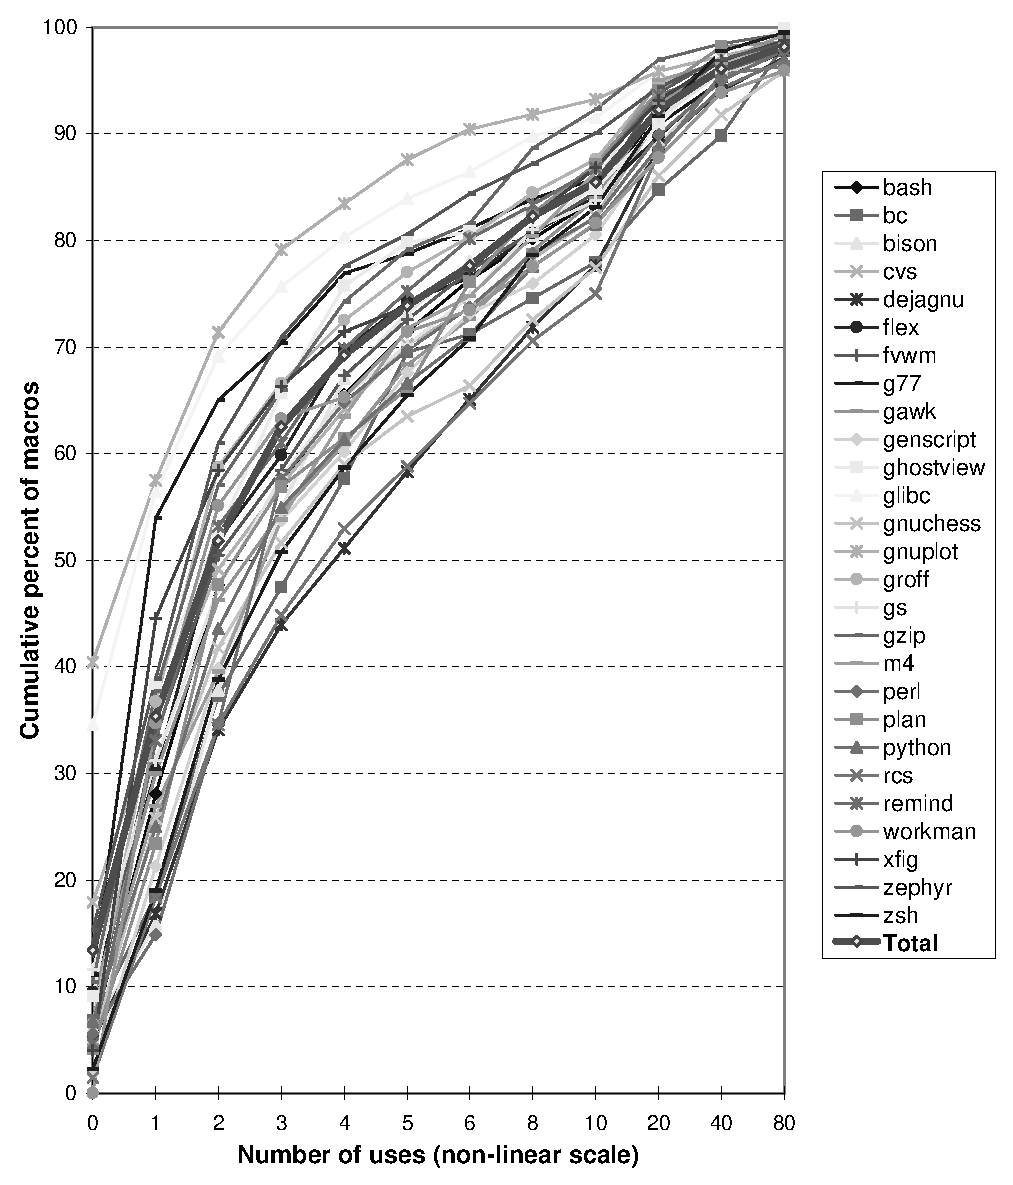
\epsfig{file=fig/use-frequency.eps,height=7.5in}}
% \caption{Number of expansions per Cpp macro.  The numbers in the
%   table represent the percentage of identifiers which are expanded a given
%   number of times or fewer.  For example, \pkg{g77} expands 65\% of its
%   macros two or fewer times.}
% \label{fig:freq-use}
% \end{figure}

\begin{figure}
\centerline{\epsfig{file=fig/cat-use-frequency.eps,height=7.5in}}
\caption{Number of expansions per Cpp macro.  The numbers in the
  table represent the percentage of identifiers which are expanded a given
  number of times or fewer.  For example, 50\% of all
  macros are expanded two or fewer times.}
\label{fig:freq-use-cat}
\end{figure}

Figure~\ref{fig:freq-use-cat} is structured as the previous figure, but it
represents the number of times that a defined name is expanded in 
the package.  About [[82\%]] of all macros were
expanded eight or fewer times.

Most packages contain a significant number of defined
macros that are never expanded\,---\,on average, 12\%.

Macros with 10 or fewer uses
cover approximately [[85\%]] of the cases.

[[Double-check all these numbers!]]
The tail of this distribution is quite long, indicating that some macros
are used very heavily.  Ninety-nine percent of macros are expanded 147 or fewer
times, 99.5\% of macros are expanded 273 or fewer times, 99.9\% are
expanded 882 or fewer times, and \pkg{python} uses {\tt NULL} (which \pkg{python}
itself defines) 4233 times.  Figure~\ref{fig:freq-use-cat} weights each macro
equally rather than weighting each macro use equally, which would weight
\pkg{python}'s {\tt NULL} 4233 times more heavily than a macro used only once
(and infinitely more than a macro never used at all).

\begin{figure}
  {\small\centerline{\begin{tabular}{|l|c|c|} \hline
 & & \multicolumn{1}{c|}{differing} \\
 & \multicolumn{1}{c|}{defs} & \multicolumn{1}{c|}{defs} \\ \hline
Null define & 2.2 & 1.0 \\
Constant & 1.5 & 1.1 \\
Expression & 1.8 & 1.4 \\
Statement & 1.7 & 1.4 \\
Type & 2.2 & 1.5 \\
Syntactic & 3.2 & 1.7 \\
Symbol & 1.6 & 1.2 \\
Unknown symbol & 1.1 & 1.0 \\
Not C code & 3.9 & 2.7 \\
Failed classification & 5.9 & 3.7 \\ \hline
Total & 1.8 & 1.3 \\ \hline
\end{tabular}

%%% Local Variables: 
%%% mode: latex
%%% TeX-master: "test-tbls"
%%% End: 
}}
  
  \caption{Summary of
    figures~\ref{fig:freq-def-cat},~\ref{fig:freq-ddf-cat},
    and~\ref{fig:freq-use-cat}.  The table is by macro name.  Add percentages?
    [[The 1.0 distinct defs for unknown symbol is surprising; it indicates
    that ti was the *same* unknown symbol in each definition (doesn't
    it?).  But a name is only in the category if none of its defs was
    recognized.  Double-check this!}
  \label{fig:freq-sum-cat}
\end{figure}

(Not sure what to say about figure~\ref{fig:freq-sum-cat}.)

\subsection{number of arguments}

\begin{figure}
\centerline{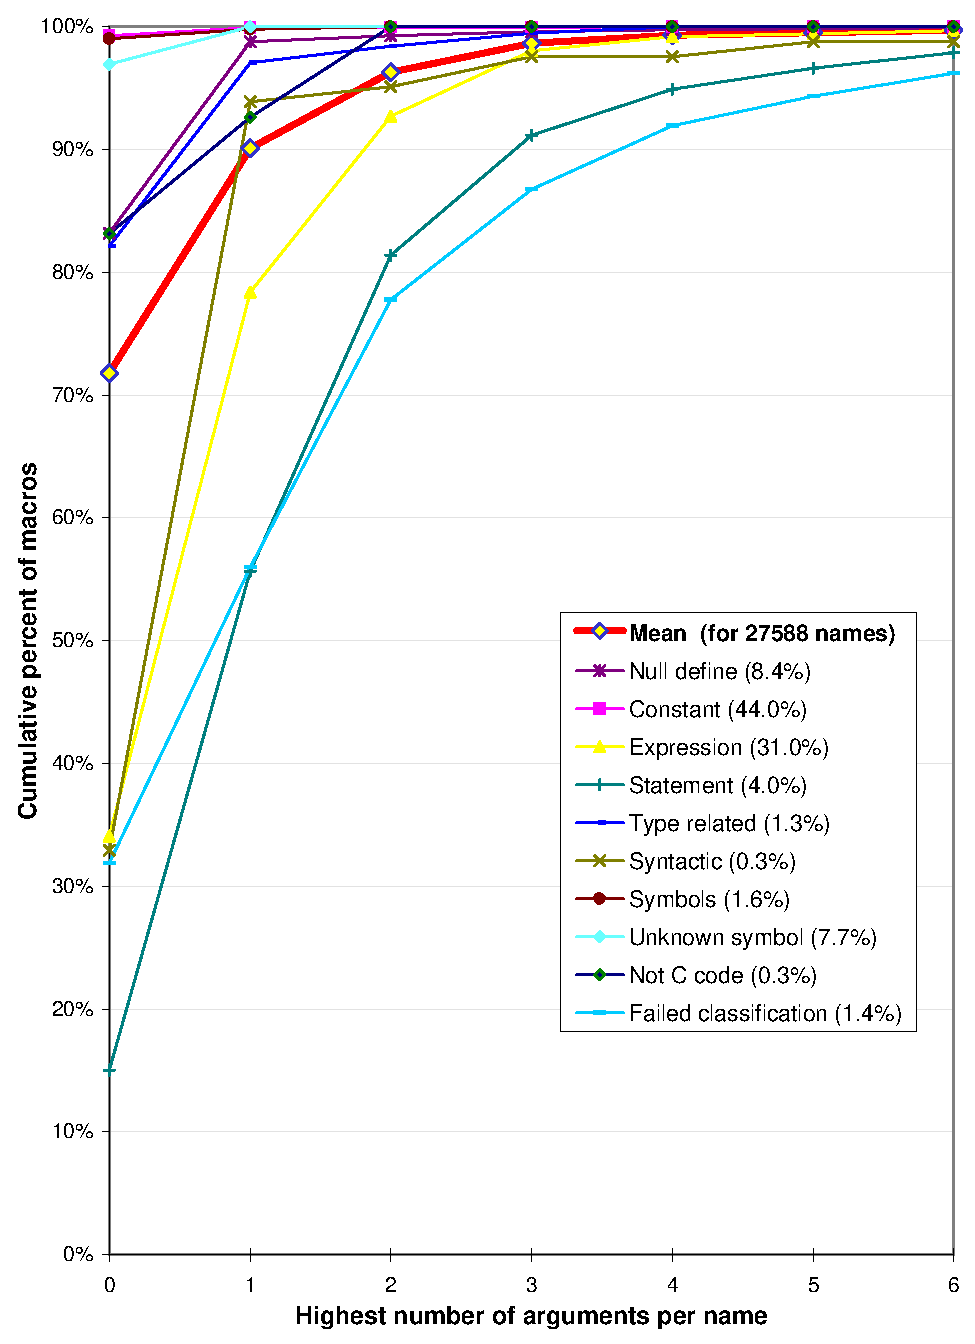
\epsfig{file=fig/cat-numargs.eps,height=7.5in}}
\caption{Is this worth including?}
\label{fig:cat-numargs}
\end{figure}

You might wonder whether macros are used like functions (taking arguments)
or like constants (taking no arguments).  We graphed that in
figure~\ref{fig:cat-numargs}.  This seems irrelevant to me; I don't see
where to fit it in, or what to say about it.

\subsection{inconsistent usage}

[[Does this general discussion belong earlier?]]

Macros have two general purposes: they can control the inclusion of lines
of code (by appearing in a {\tt \#if} condition that controls that line) or
can change the text of a line (by being expanded on that line).  Each of
these uses can often be modeled by C++ language features -- conditionals or
(for certain types of substitution) consts and inlines.  But when a macro
is used in both ways, then there's no one C++ language feature.
(Additionally, it's harder to understand and to analyze a macro that's used
in both ways than one that is only used in one way or the other.)
[[Or maybe more is going on, or conceptually different uses have been
merged into a single name.]]

    We split macro uses into three categories:  
\begin{itemize}
\item
  uses in C code, where the macro's expansion controls textual
            replacement
\item
  uses in {\tt \#if}, {\tt \#ifdef}, {\tt \#ifndef}, {\tt \#elif} conditions
\item
  uses in a macro body, which eventually bottom out to one of the
            others (unless that macro is never used...)
\end{itemize}

\begin{figure}
{\small
  \setlength{\tabcolsep}{.25em}
  \begin{tabular}{|l|r|}\hline
Code & 62.9%\\\hline
Code, macro & 12.3%\\\hline
Cond. & 6.4%\\\hline
Cond., macro & 0.3%\\\hline
Macro & 5.0%\\\hline
Code, cond. & 1.7%\\\hline
Code, cond., macro & 0.7%\\\hline
No uses & 10.9%\\\hline
Total & 22929 & (100%)\\\hline
\end{tabular}
%
}
\caption{Where macros are used: in C code, in macro definition bodies, in
  conditional tests, or in some combination thereof.  The numbers don't sum to
  100\% because of rounding.  It might perhaps be interesting to see this
  broken down by category.}
\label{fig:where-used}
\end{figure}

      We discarded uses in CPP conditionals whose only purpose was to
        prevent redefinition.  More specifically, if the condition tested
        only definedness, the next line defined the macro just tested, and
        the line after that ended the CPP conditional.  This is a bit
        overrestrictive, but conservative, and in practice quite accurate.
        
        Uses in a macro body generally are intended to be used however the
        containing macro is.  Since those uses also appear in
        figure~\ref{fig:where-used}, we did not attempt to track each such
        use in a body to some macro's appearance in either code or a
        conditional.  
        A definition isn't a use of the macro being defined, only of those
        in the body.  Since those are uses, 12\% is a lower bound on those
        that never affect the code.
        It would be reasonable to assign the 5.4\% that are macro only, to
        the other categories on a pro rata basis.
        Thus, the interesting categories are "code",
        "conditional", "code and conditional", and "no use".

      Macros are used more frequently to expand code than to control its
        inclusion, by a factor of ten to one.  (However, each inclusion use
        can control many lines of code; see the dependence section, below.)
The dominant usage was in C code only; these uses
do not, therefore, have any affect on conditional compilation (for example).

[[Move this to the previous section, and reference back to it.]]
      A surprising number -- nearly 12\% -- of macros defined in a package
        are never used at all.  Occasionally [[find a concrete example of
        this]] this is a result of shipping a 
        standard set of headers with the package -- it's like a library for
        that development team, but one that can't be counted upon to exist
        everywhere, so it has to be provided.  For gnuplot, over 40\% of
        macros are never used because the package's support for several
        terminal types, such as tgif, is unfinished (and thus unused).
        Even discounting that package, though, the numbers are remarkably
        high.  We would be surprised if one in eight functions and
        variables in a package were never used, not even in testing code.
        [[Do we have any idea what fraction this is in practice?]]
        (The percentage of macros defined in libraries/standard header
        files which are never used in the code is enormous, but that is
        expected.)

      The potentially problematic uses are those for which a macro appears
        both in code and in a conditional; these comprise only 3.4\% of all
        macro names.

      Across packages, there is heavy variation.  Packages which use
        the preprocessor sparingly are as likely to have a high percentage
        of mixed usage as packages which make heavy use of CPP.  (There is
        a very slight tendency for the less aggressive packages (i.e.,
        those lower on the lists in figures~\ref{fig:directives-breakdown}
        and~\ref{fig:categorization}) to have more uses in code, fewer uses
        in conditionals, and fewer macros that are never used.)

In general, packages use macros either to direct conditional compilation or
to produce code, but not for both purposes; this separation of concerns
makes the source code easier to understand.  Only 3.4\% of macros expand in
both code and conditional contexts (plus a similar percentage of those used
in other macros). 
Conditional usage is rare in general; conditional compilation accounts for
half of Cpp directives but only 7.1\% of macro usage (plus the categories just
listed above).  But each use in a conditional can have a large effect on
the system.


\subsection{Mixed usage in conditional control}

\begin{figure}
\centerline{\epsfig{file=fig/ccd-categories.eps,height=7.5in}}
\caption{CCD categories.  [[Reorder according to order in text.  Perhaps
  change legend to 2 or 3 columns, underneath.]]}
\label{fig:ccd-categories}
\end{figure}


    Conditionals are used to check for a bunch of things (examples); but a
      single conditional generally checks just one of these categories.  We
      counted the number in each, and also the number that checked symbols
      falling in multiple categories.

    Few mixed categories.

    Lots of variation overall.

    The macros with mixed usage (especially here, but also in the previous
      section) are akin to Krone \& Snelting's anomalous macros that
      interfere in the lattice.  But we found more than they seemed to!
      [[Did we analyze the package in which they found their problem?]]
      
      Each symbol is assigned to a category; if all symbols in a
      conditional guard are in the same category, then the conditional test
      is assigned to that category; otherwise, the conditional text is
      given category ``mixed.''  The categorization is based on the macro
      {\em name} alone; but this works because of naming conventions for
      various types of macro use.  (We examined a bunch of macro names
      (compiled from a list of all macro names appearing in conditionals)
      to refine our heuristics.)


{The following categories are based on macro names:

\begin{description}
%% See ccd_lexical_category in em_analyze for the routines
%% which implements these heuristics

\item[Package-specific] 
  These symbols are specific to the given package.  They do not fit any of
  the other categories.

\item[Portability, machine]
  These symbols name the operating system or machine
  hardware (e.g., \texttt{sun386} or \texttt{MACINTOSH}).
      
\item[Portability, feature] These symbols describe specific parameters
      or capabilities of the target machine or operating system (e.g.,
      \texttt{BYTEORDER}, \verb|BROKEN_TIOCGWINSZ|).  
      
%      These symbols are different from ``portability, machine'' because
%      they may correspond to multiple machines or architectures.

\item[Portability, system macro]
  These symbols are commonly defined constants or
  pseudo-inline functions in system or language libraries (e.g.,
  \verb|O_CREATE|, \texttt{isalnum}, or \verb|S_IRWXUSR|).

\item[Portability, language or library]
  These symbols are predefined by a compiler, defined by a standard
  library, or defined by the package as part of the build
  process to indicate existence of compiler, language, or library features
  (e.g., \texttt{GNUC}, \texttt{STDC}, or \verb|HAS_BOOL|).

\item[Miscellaneous system]
  These symbols are reserved (i.e., they begin with two underscores) and do
  not fit any other category.
      
\item[Debugging]
  These symbols control inclusion of debugging or tracing code.  The macro
  names include \texttt{DEBUG} or \texttt{TRACE} (or both).
      
\item[Multiple inclusion prevention]
  These guards encompass an entire file to ensure that the enclosed code is
  seen only once per translation unit by the compiler.  Such guards are
  indicated by convention with a trailing \verb|_H| or \verb|_INCLUDED| in the macro name
  they check.
\end{description}


The below three categories consider the entire guard or the context of
the directive.  These categories have precedence over the above name-based
heuristics:

\begin{description}
\item[Commenting] These guards either definitely succeed and
  have no effect as written (e.g., \texttt{\#ifdef 1}), or definitely fail
  and unconditionally skip a block (e.g., {\tt \#ifdef (0 \&\&
    \verb|OTHER_TEST|)}).  These guards are used to comment out code or to
  override other conditions (e.g., to unconditionally enable a previously
  experimental feature).
      
\item[Redefinition suppression] These guards test non-definedness of
  symbol, and control only  a definition of the same symbol, thus avoid preprocessor
      warnings about a redefinition of a name (e.g., \texttt{\#ifndef
      FOO} followed by \texttt{\#define FOO ...} and \texttt{\#endif}).
    
    The purpose is to provide a default value used unless another part of
    the system, or the compilation command, specifies another value.

\item[Mixed categories] These guards test multiple symbols
      which independently fall into different categories (e.g.,
      {\tt \#if defined(\verb|STDIO_H|) || \verb|SYSV_SIGNALS|}).

\end{description}

%%% Local Variables: 
%%% mode: latex
%%% TeX-master: "emp-use-2"
%%% End: 
}


\section{Dependences}
\label{sec:dependence}
\label{sec:last-content-section}

 Two types of dependence:  control/inclusion, and substitution/expansion
     This includes macros which control its inclusion via conditional
     compilation, macros that are invoked on the line, and macros that
     control the definitions of, or are called by, directly invoked macros

 Explain this.  Explain how we compute it transitively.
 
 The dependence charts omit Emacs and Mosaic; the full dependence
 information for each overran our computer's virtual memory.  This was in
 part due to dependences in libraries; the Motif library is a particular
 problem.  (We did compute dependence information for Plan, which is the
 third of our 30 packages which uses the Motif library.)  So these numbers
 are smaller than they might be with more complete information.

Note that we are reporting on may dependences, not only must dependences.
Mention some dependence types from notes ``must and may dependences'' section.

\subsection{line dependent on many macros}

\begin{figure}
\centerline{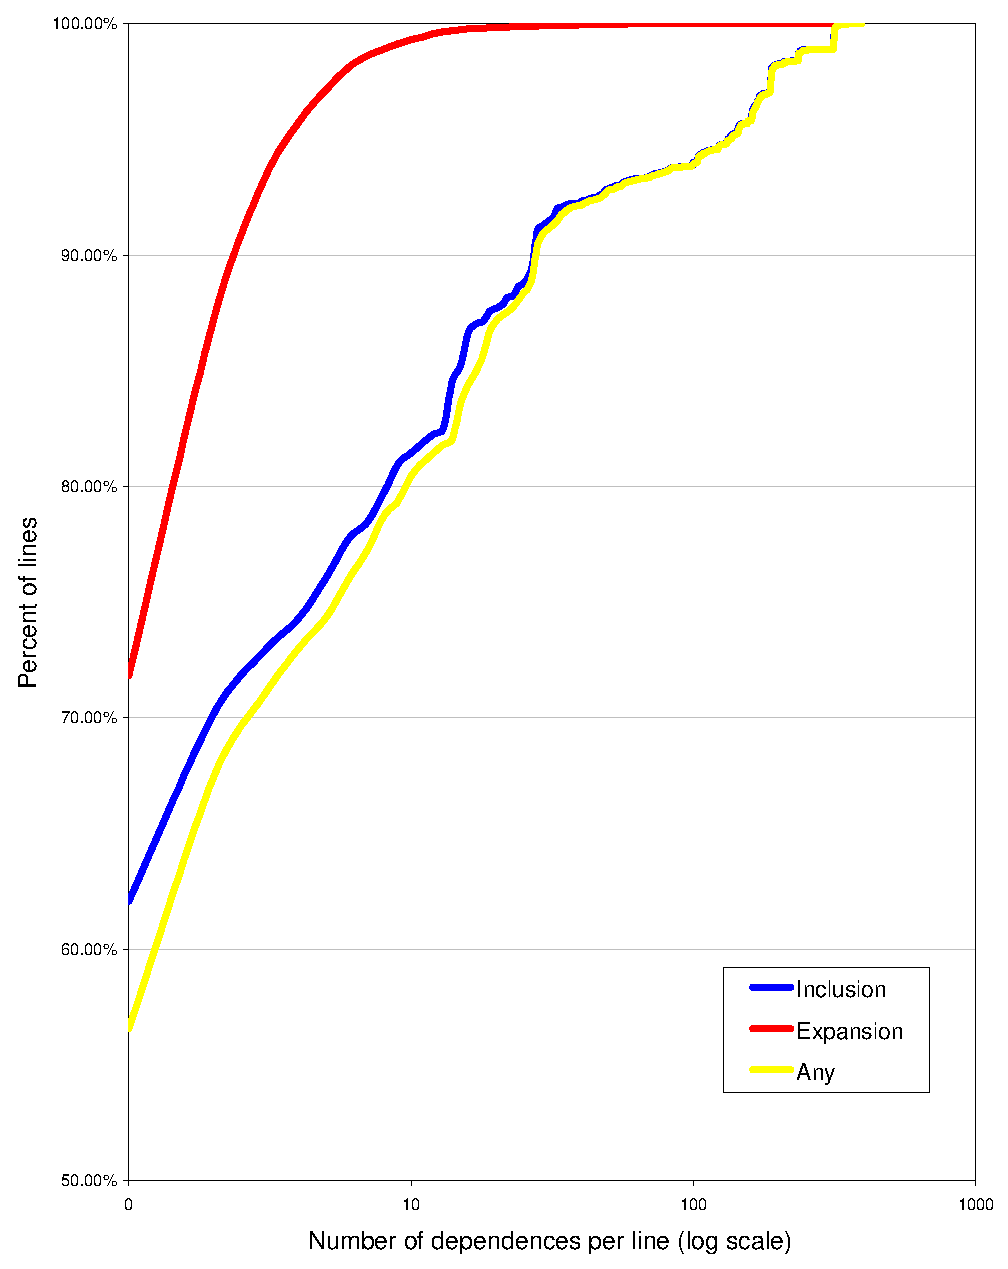
\epsfig{file=fig/dep-byline.eps,height=7.5in}}
\caption{dep-byline for 28 packages.
The log scale is shifted by unity in order to place 0 on the scale; that
is, we added 1 to each of the x axis values, before plotting, then
relabeled ``1'' as ``0''.}
\label{fig:dep-byline}
\end{figure}


    [Gloss over what kind of line; I think it's a physical line, but each
      physical line is coalesced with other parts of its logical line for
      the purpose of computing dependence info.]

    We computed, for each line, the number of macros it depends on.

There are two types of dependence:  control and expansion.  Make sure we
have good names for these!

    Describe the matrix:  ExE=E, Cx?=C, ?xC=C; plus, we sum across
      conditional compilations and alternate definitions.

    
      58\% of lines have no dependence on macros at all.  (Most lines that
      don't expand any macros and appear in C files fall into this category.)

    Overall, 28\% of lines expand a macro -- that's quite a few.

    5\% of all lines depend on at least 134 macros.

    On average, each line is expansion-dependent on .040 macros,
      inclusion-dependent on .31 macros, and any-dependent on .34 macros.
      (These numbers don't add up because a line may be both expansion and
      inclusion dependent on a macro, but that macro is only counted once
      in the "any dependence" number.)
      
      One line of gcc is expansion-dependent on the expansions of 187
      macros.  (This is an outlier: of the 297,760 [[huh?? this doesn't
      jibe with figure~\ref{fig:packages}!!  double-check]] lines in gcc,
      only 13 are expansion-dependent on more than 100 macros -- all of
      which fall in the range of 159 to 187 such dependences.)

        It's this one, whose mere appearance in the final source is
        dependent on 182 macros (not such an outlier: over 10,000 lines are
        inclusion-dependent on more than that many macros):

        gcc-2.7.2.1/explow.c:430: dependences incl=182; exp=187; either=356
              \verb|LEGITIMIZE_ADDRESS| (x, oldx, mode, win);

        \verb|LEGITIMIZE_ADDRESS| is defined 30 times in gcc, and one randomly-selected
        definition was 37 lines long (and chock full of other macro invocations).
        [[be more specific, or say ``many of them dozens of lines long'']]

\subsection{macro controlling many lines}

    We combined these charts for the different packages, because the shapes
      of each were quite similar for each package.  In order to permit
      combining charts across quite different package sizes, we computed
      values that were percentages of package size.

   \subsubsection{expansion}

\begin{figure}
% This works, but the figures are upside-down.
% \centerline{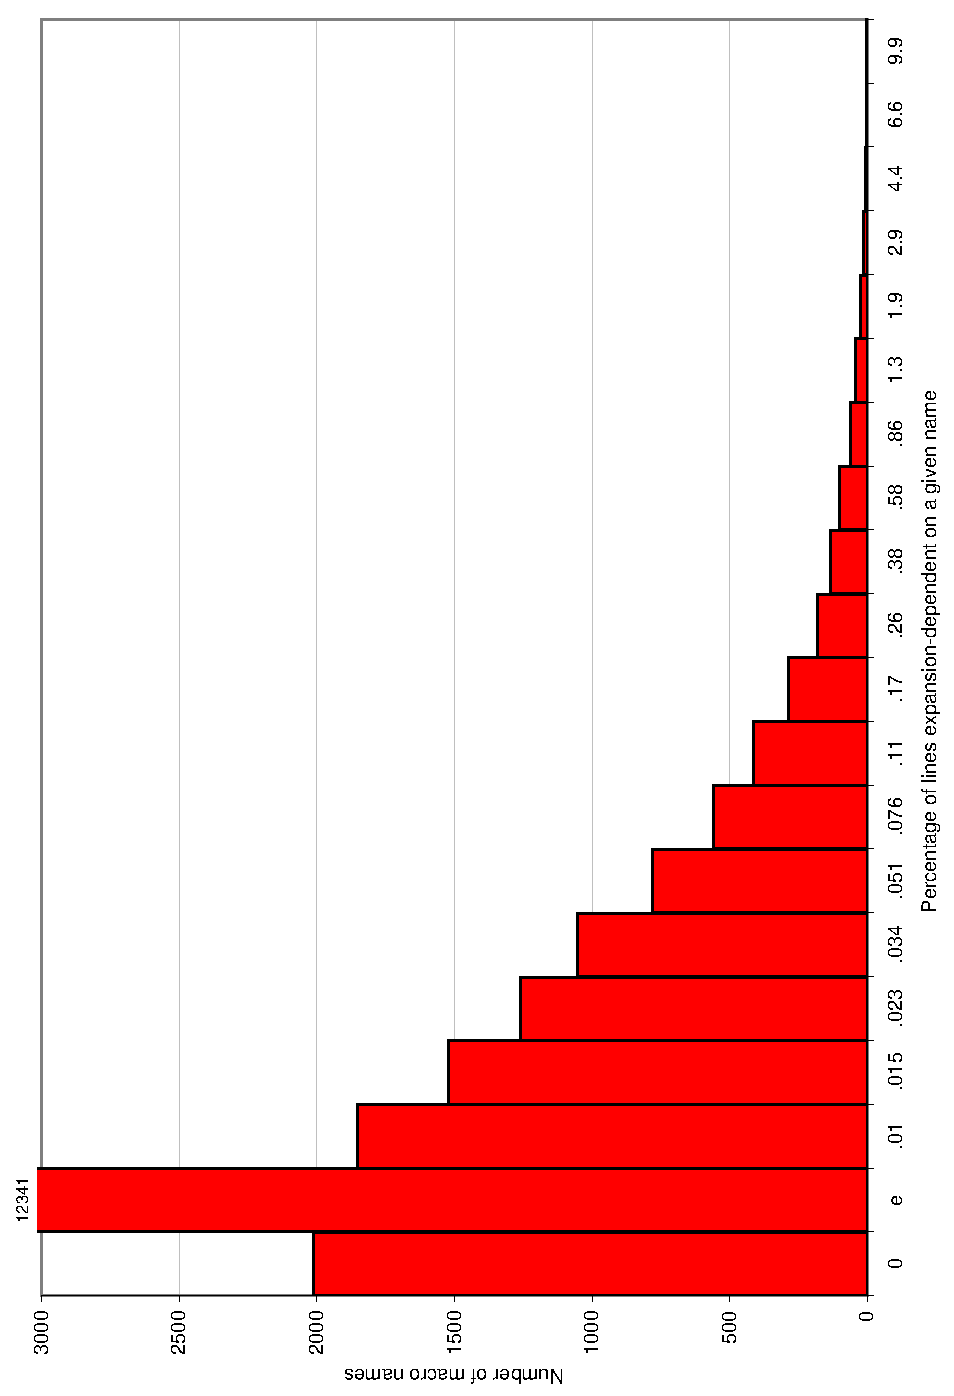
\epsfig{file=fig/exp-dep-bymacro.eps,angle=90,height=3.75in}}
% \centerline{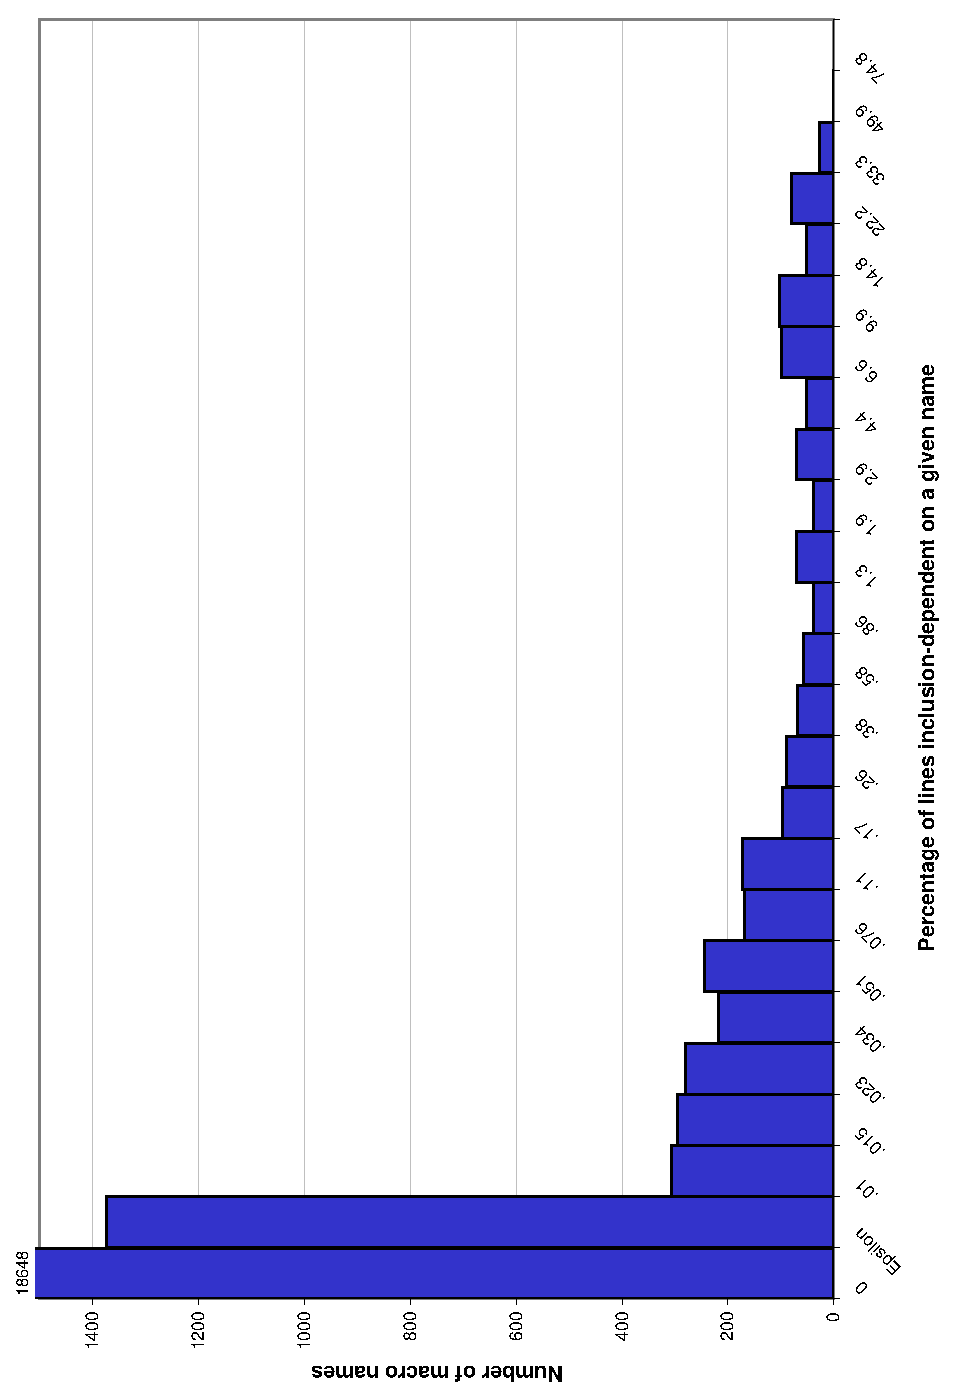
\epsfig{file=fig/incl-dep-bymacro.eps,angle=90,height=3.75in}}
% Can't use ``height'' when rotating by -90 or +270; I don't know why.
\centerline{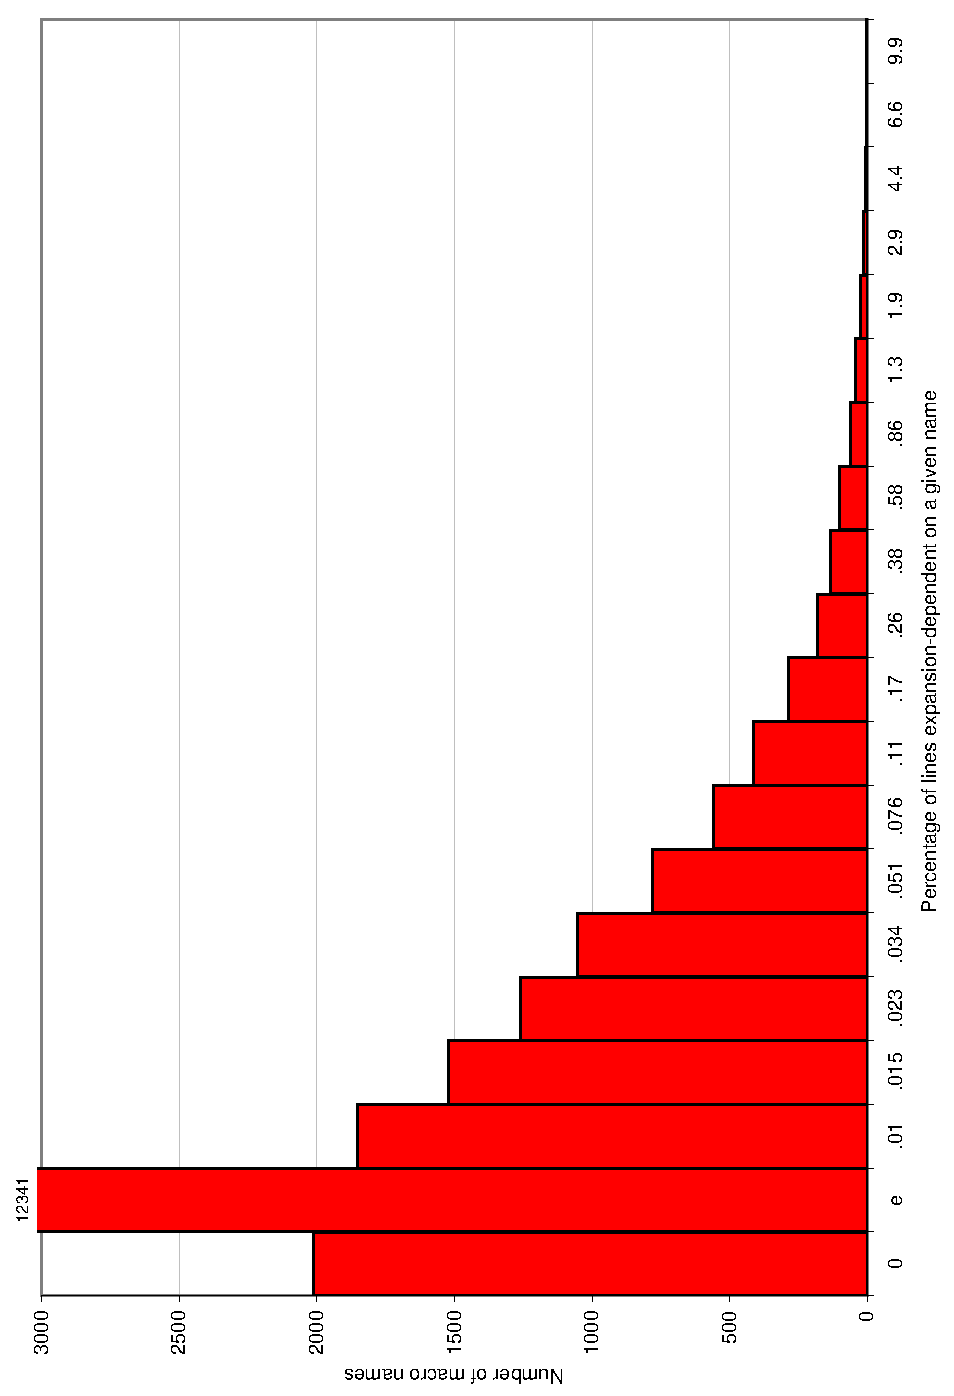
\epsfig{file=fig/exp-dep-bymacro.eps,angle=270,width=.9\linewidth}}
\bigskip
\centerline{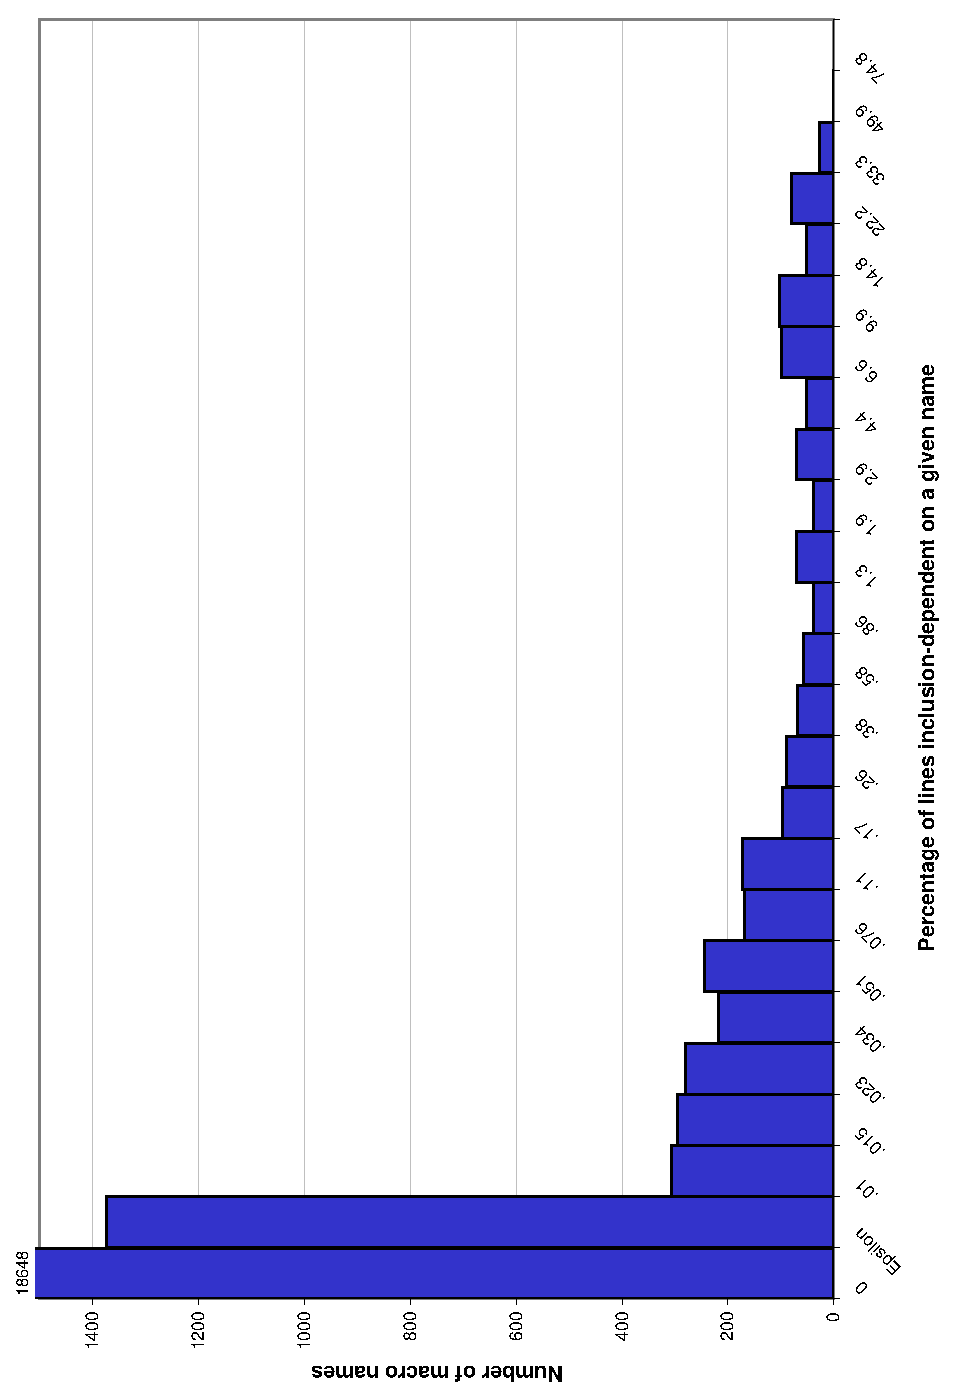
\epsfig{file=fig/incl-dep-bymacro.eps,angle=270,width=.9\linewidth}}
\caption{dep-bymacro for 28 packages.
  Each bar represents all macros that control less than the bar label
  percent of the lines in its package (but more than the previous label).
  For instance, the .17 bar in the red chart indicates that there are 286
  macros that each control between .11\% and .17\% of the entire package
  containing that macro.  The maximum falls in the last bucket specified
  (i.e., the first bucket off the chart is the first empty one).}
\label{fig:dep-bymacro}
\end{figure}

Practically every {\tt \#if} line (which accounts for about half of the
conditional compilation lines) expands a macro.  (Some don't, for instance
when testing which character set is being used on the compiling machine.)

        This exponential decay indicates that, as expected, there are more
          macros which control just a few lines and fewer macros that
          control a lot of lines.

        Outliers (> 6\% of all lines expand):
          int in gcc (14.85\% !)
          NULL, ANY, object in python

        Above 5\%: 
          SvANY in Perl
          const in RCS
          ip in workman -- bogus, as defined just twice, then undefined;
                  most places it is a formal parameter and out of the scope
                  of the macro definition.
          ArgCount, Args in xfig (like argc, argv)
          rtx in gcc (defined to int or int*)

        Overall, for these top 10:  6 types, 1 constant, 3 expressions

   \subsubsection{inclusion}

        For each package, the graph is bimodal (so much so that this even
          shows up a bit on the combined chart; it's more marked in the
          individual packages, I think).  Most macros control inclusion of
          no, or very few, lines; but quite a few control a substantial
          fraction of the package (around 10\%).

        All the heaviest dependences are on header files (for instance,
          \verb|H_PERL| controls inclusion of over 53\% of Perl's lines).

        [It would have been interesting to run these numbers for everything
          but include file multiple inclusion prevention macros.]


\subsection{CPPP experiment}

    [After the above, this experiment doesn't sound like such a smart thing
      to try any more; its results certainly aren't unexpected.]

    We had noticed in our programming that a particularly heavy use of the
      preprocessor is to handle multiple dialects of a language.  These uses
      tend to be less structured:  they don't have a simple pattern.  And
      this work must be done in the preprocessor:  there's no hope of
      integrating it into the language.  So we performed an experiment to
      see whether standardizing on a single language would reduce
      dependences, failed classifications, etc.

    We built a CPPP partial evaluator (called cppp) which, given a set of
      macros known to be defined or undefined (and, optionally, their
      expansions), eliminates all possible CPP conditionals.  We defined
      all the macros that can be depended on if using ANSI standard C or
      C++ (including prototypes and booleans) with POSIX-compliant
      libraries, preprocessed all the source (and 
      all library header files), and reran our experiments.

    The results were disappointing:  while some numeric measures of how
      complicated the resulting program's dependences are decreased, most
      remained at about their previous level.  The number of multiple
      definitions of macros, and the number of failed classifications, did
      not decrease as much as anticipated.

    From this we can conclude that there is no one obvious single point of
      attack:  even eliminating what seems most prevalent to us doesn't
      make a sufficient difference.



\section{Related work}
\label{sec:related}


We could find no other empirical study of the use of the C preprocessor nor
any other macro processor.  However, we did find guidance on using C macros
effectively and tools for checking macro usage.

Carroll and Ellis state that ``almost all uses of macros can be eliminated
from C++ libraries''~[p.~146]{Carroll95}.  They list eight categories
of macro usage and explain how to convert them into C++ mechanisms.  They
do not discuss automatic conversion, but focus on instructing the software
engineer on better ways to do Cpp-like things.

Similarly, a number of organizations provide hints about effective ways to
the use the C preprocessor.  The GNU documentation discusses
a set of techniques including simple macros, argument macros, predefined
macros, stringization macros, concatenation macros, and undefining and
redefining macros.  It also identifies a set of ``pitfalls and subtleties
of macros''; these are much like some of the problems our analysis tool
identifies.

We discovered that these categorizations sometimes focussed on constructs
that don't happen very often or missed ones that are actually frequent.
Our effort not only categorizes problems, but it also determines the
frequency of appearance of those problems and discovers other idiosyncratic
uses.

A number of tools check whether specific C programs satisfy particular
constraints.  The lint program checker [[reference]]
checks for potentially problematic uses of C\@.  
[[This is irrelevant, unless you're going to claim that it does a worse job
than one would like.]]
The implementation of lint
is complicated by the fact that it tries to replicate significant functions
of both the C compiler and the preprocessor.

LCLint performs many of lint's checks and also
allows the programmer to add annotations which enable additional
checks~\cite{Evans-pldi96,Evans-fse94}.
LCLint optionally checks function-like
macros\,---\,that is, those which take arguments\,---\,for
macro arguments on the left hand side of assignments, for statements
playing the role of expressions, and for consistent return types.
%\begin{quote}
%$\ldots$ a parameter to a macro may not be used as the left hand side
%of an assignment expression $\ldots$, a macro definition must be
%syntactically equivalent to a statement when it is invoked followed by
%a semicolon $\ldots$, the type of the macro body must match the return
%type of the corresponding function $\ldots$\footnote{From Section 8 of
%David Evans's LCLint User's Guide, Version 2.2 (August 1996); larch-www.lcs.mit.edu:8001/\discretionary{}{}{}larch/\discretionary{}{}{}lclint/\discretionary{}{}{}guide/\discretionary{}{}{}guide.html}
%[FIX: That footnote should really be a reference instead.]
%\end{quote}
%[Fix: that quotation is really easy to nitpick:
% 1) assignment parameters is fine (just turn into a reference argument) but
%    assignment of non-parameters that aren't at global scope is quite bad.
% 2) in x=foo(); we do NOT want foo() to be a statement
% 3) a macro doesn't have a single type, but may have many polymorphic types
%Should we mention these things?  I don't want to seem nitpicky or petty.]
LCLint's approach is prescriptive: programmers are encouraged not to use
constructs that might be dangerous, or to change code that contains such
constructs.  We are more interested in analyzing, describing, and
automatically removing such uses so that tools can better process existing
code without requiring human interaction or producing misleading results.

%% FIX: If we could also list the platforms for which each can compile,
%% that would be great, but I doubt the benefit is worth the effort for now

Krone and Snelting use mathematical concept analysis to determine the
conditional compilation structure of code~\cite{Krone94}.  They determine,
for each line, which preprocessor macros it depends upon, and display that
information in a lattice.  They do not determine how macros depend upon one
another directly, only by their nesting in {\tt \#if}, and the information
conveyed is about the program as a whole.


[[Expand; relocate in this section?]]
A limited number of tools do exist to assist software engineers to
understand code with containing Cpp directives, such as debuggers that can
call {\tt \#define}d functions and editors that support viewing one
particular configuration of the code.



\section{Conclusions}
\label{sec:conclusion}

[[Grist for conclusion: These data demonstrate that multiple definitions of
symbols is not numerically frequent; even more importantly, the definitions
of a symbol tend to be compatible, as shown in
section~\ref{sec:inconsistent}.]]


% \subsection{Who cares?}
\subsection{Relevance of the results}

[[This is the place to recap the various sections, giving the highlights of
each.]]

The results of this research are of interest to language designers, tool
writers, programmers, and software engineers.

Language designers can examine uses of the macro system's extra-linguistic
capabilities to determine what programmers consider missing from the
language.  Future language specifications can support (or prevent!)\ such
practices in a more disciplined, structured way.

% [[[Think more about this:  Also, how do language choices lead to more/less
% tightly integrated (as opposed to open, component-based) environments?
% E.G., no need for \verb|__LINE__| in Java?]]]

Programming tool writers, too, need to understand how Cpp is used, for that
sheds insight on the sorts of inputs that will be provided to the tool.  By
coping with the most common constructs, the tool can provide relatively
good coverage for low effort.  By identifying problematic uses, much better
feedback can be given to the programmer, who can be more effective as a
result.  The analysis results also indicate the difficulty of processing [wc]
preprocessor directives; before these analyses, we did not know whether the
task was so trivial as to be uninteresting, so difficult as to be not worth
attempting, or somewhere in between.

The analyses are of interest to programmers who wish to make their code
cleaner and more portable, and can help them to avoid constructs that cause
tools (such as test frameworks and program understanding tools)
to give incomplete or incorrect results.

% Also, learn weird new Cpp tricks!

Finally, our results are of interest to software engineers for all of the
above reasons and more.  Since this is the first Cpp usage study of which
we are aware, it is worth performing simply to determine whether the
results were predictable a priori; we did in fact discover a number of
interesting features of our suite of programs.


\subsection{Making C programs easier to understand}

The combination of C and Cpp makes a source text unnecessarily difficult to
understand.  A good first step is to eliminate Cpp uses where an equivalent
C or C++ construct exists, and to apply tools to explicate the remaining
uses.  Here we discuss a few approaches to solving this problem by
eliminating the source of confusion rather than applying tools.  We do not
seriously consider simply eliminating the preprocessor, for it provides
conveniences and functionality not present in the base language.

Since many of the most problematic uses of Cpp provide portability across
different language dialects or different operating environments,
standardization can obviate many such uses.  Canonicalizing library
function names and calling conventions makes conditional compilation less
necessary and incidentally makes all programs more portable, even those
which have not gone to special effort to achieve portability.  This
proposal moves the responsibility for portability (really, conformance to a
specification) from the application program into the library or operating
system, which is a reasonable design choice since many application programs
rely on a much smaller number of libraries and run on relatively few
operating systems.

Likewise, the most common single cause [[Really?  I'm not sure I believe
that without qualification]] for Cpp directives would be eliminated if the
C language and its dialects had only a single declaration syntax.  Because
most C compilers, and all C++ compilers, accept ANSI-style declarations,
much support for multiple declaration style may have outlived its
usefulness.  [[On the other hand, K\&R support was just *added* to some
mature, popular package (zsh?) recently.]]  We are investigating the effect
on our statistics (and program understandability) of ``partially
evaluating'' a program source by specifying the definedness and values of
some Cpp identifiers.

Some Cpp directives, such as {\tt \#include}, can be moved into the
language proper; this would also eliminate the need for Cpp constructs that
prevent multiple inclusion of header files.  Likewise, compilers that do a
good job of constant-folding and dead code elimination can encourage
programmers to use language constructs rather than relying on the
guarantees of an extra-linguistic tool like Cpp.\footnote{Interestingly,
  the issue seems to not be whether compilers do the appropriate
  optimizations, but whether programmers have confidence that the
  optimizations will be performed; if unsure, programmers will continue to
  resort to Cpp, since certainly a compiler cannot generate code for source
  that it does not ever even see (because Cpp has already stripped it
  away).}

Common Cpp constructs could be replaced by a special-purpose syntax.  For
instance, declarations or partial declarations could be made explicit
(perhaps first-class) objects; similar support could be provided for
repetitive constructs and dynamic scoping.  Manipulations of these objects
would then be performed through a clearly-specified interface rather than
via string and token concatenation, easing the understanding burden on the
programmer.  Such uses would also be visible to the compiler and could be
checked and reasonable error messages provided.  The downside of this
approach is the introduction of a new syntax or new library functions which
may not simplify the program text and which cannot cover all cases, only a
few specified ones.

[[Add a hygenic macros reference somewhere.]]

An alternative approach which avoids the clumsiness of a separate language
of limited expressiveness is to make the macro language more
powerful\,---\,perhaps even using the language itself via constructs
evaluated at compile time rather than run time.  (The macro systems of
Common Lisp and Scheme, and their descendants~\cite{WeiseC93}, take this
approach.)  An extreme example would be to provide a full-fledged
reflection capability.  Such an approach is highly general, powerful, and
theoretically clean; it circumvents many of the limitations of Cpp,
though it does not necessarily support all of Cpp's low-level features.
However, this approach may degrade rather than improve programs
understanding.  As difficult as it may be to determine what output a
macroless program produces, it can be just as difficult simply to determine
the text of a program which uses such macros.  (This is also a problem with
meta-object protocols, aspect-oriented programming, and intentional
programming, all of which permit the programmer to specify transformations
on other parts of the source code.  In practice, such systems are used in
fairly restricted ways, perhaps because other uses would be too
complicated.)  A dialog among users, compiler writers, tool writers, and
language theorists is necessary when introducing a feature in order to
prevent unforeseen consequences from turning it into a burden.


%% See slide 15 and its notes from Mike's quals talk.
\subsection{Future work}
 
These results suggest a wide variety of future avenues for research, both
in terms of expanding our understanding of uses of the preprocessor in
practice and in addressing the issues identified by this study.

A straightforward refinement that we are pursuing examines macro uses to
aid this categorization.  (For example, a macro used where a type should
appear can be inferred to expand to a type; a macro used before a function
body is probably expanding to a declarator.)

Further analysis of the conditional
compilation structure (in the style of Krone and Snelting~\cite{Krone94})
and of the macros with free variables (essentially achieving dynamic
scoping) is needed to see which of the roughly 29\% of expression macros
should be easy to convert to C++ language features such as constants or
enumerated values.

  We are concerned with how it {\em could} be used, not just how it {\em
  happens} to be used.  That's why we can't take the easy out.  But it
  would be interesting to look at uses, which would let us infer the {\em
  intended} use (if not all {\em possible} uses).  We are actively pursing
  this line of research.


No libraries (eg, \pkg{glibc}), as they're too different than applications.
No C++.\footnote{Preliminary results indicate that many
  C++ packages rely heavily on Cpp, even when C++ supports a nearly
  identical language construct, probably due to a combination of trivial
  translations from C to C++ and of C programmers becoming C++ programmers
  without changing their habits.}

``As with all benchmarks, there is the question of how representative this is.''

Variations among packages:
 * The C language has changed.  How do newer packages compare with older ones?
 * How do PC packages compare with Unix packages?  Less pressure to make it
   work on many platforms, because there aren't as many?
 * Correlate human perceptions of good or bad preprocessor use with what my
   tool says.
 * What's special about GNU programs?  Compare GNU to non-GNU?
 * Applications vs. libraries?  Get more libraries, or eliminate the current
   ones.




% Not really right:  Don't want the ``References'' section head to be small.
{\small \bibliography{evil}}

\end{document}
